%!TeX spellcheck = en-GB

%Basics
\documentclass[aps, prb, a4paper, english, 12pt, onecolumn, longbibliography, amsmath, amssymb, colorinlistoftodos, floatfix, svgnames]{revtex4-2}
\usepackage[utf8]{inputenc}
\usepackage{babel}

%Symbols and scientifics
\usepackage{amsmath, amsfonts, amssymb, bm}
\numberwithin{equation}{section}
\usepackage{physics}
\usepackage{mathtools}
\usepackage{siunitx}
\sisetup{
	per-mode = power,
	round-mode = figures,
	round-precision = 3,
	scientific-notation = false,
	output-decimal-marker = {.},
	exponent-product = \times,
	separate-uncertainty = true,
	uncertainty-separator = \ ,
	output-product = \cdot,
	quotient-mode = fraction,
	range-phrase = -,
	range-units =  single,
	inter-unit-product = \ensuremath{{\cdot{}}},
%	number-unit-product = \ ,
	multi-part-units = single,
	alsoload = synchem,
	alsoload = addn
}
\DeclareSIUnit\atm{atm}
\usepackage{chemfig}
\usepackage{tikzorbital}

%Appendix, TOC and Bibliography
\usepackage{appendix}
\renewcommand\appendixtocname{Appendices}
%\usepackage[nottoc]{tocbibind}
\usepackage[lastpage,user]{zref}

%Figures
\usepackage{float}
%\setlength{\textfloatsep}{5.0pt plus 2.0pt minus 4.0pt}
%\setlength{\intextsep}{5.0pt plus 2.0pt minus 2.0pt}
\usepackage{xcolor} % Required to specify font color
\usepackage{graphicx}
\usepackage{setspace}
\usepackage{caption}
\usepackage{subcaption}
\usepackage[format=plain,
            labelfont={bf,it,footnotesize},
            textfont={it,footnotesize}]{caption}
\captionsetup{font={stretch=1}}
\usepackage[verbose]{wrapfig}
\usepackage[a4paper, centering, rmargin=2.5cm, tmargin=2.5cm, lmargin=2.5cm, bmargin=2.5cm]{geometry}
\usepackage{etoolbox}
\usepackage{verbatim}
\usepackage[space]{grffile}
\usepackage[final]{pdfpages}
\usepackage{array}
\usepackage{multirow}
\usepackage{dcolumn}
%\usepackage{animate}
\usepackage{fontawesome}
\usepackage[european]{circuitikz}
\usepackage{pdflscape}
\usepackage{pgfplots}
\pgfplotsset{width=10cm, compat=newest}
\def\axisdefaultwidth{10cm}
%\usepgfplotslibrary{external}
\usepgfplotslibrary{units}
%\tikzexternalize
\usepackage{pgfgantt}
\newcounter{myWeekNum}
\stepcounter{myWeekNum}
%
\newcommand{\myWeek}{\themyWeekNum
    \stepcounter{myWeekNum}
    \ifnum\themyWeekNum=53
         \setcounter{myWeekNum}{1}
    \else\fi
}
%

%Header footer
\usepackage{fancyhdr}
\pagestyle{fancy}
\lhead{C. V. Sørensen \\ R. K. F. Wiuff}
\chead{Quantum Transport in NPG\\DTU Department of Physics}
\rhead{May \nth{1}\\2019}
\cfoot{Page \thepage\, of \zpageref{LastPage}}
\renewcommand{\headrulewidth}{0.4pt}
\renewcommand{\footrulewidth}{0.4pt}

%Text tools
\usepackage{listings}
\usepackage{parcolumns}
\usepackage[super]{nth}
\usepackage[normalem]{ulem}
\usepackage{import}
\usepackage{url}
\usepackage{lipsum}
\usepackage{microtype}
\usepackage[pdfencoding=auto, psdextra]{hyperref}
\hypersetup{
	colorlinks   = true, %Colours links instead of ugly boxes
	urlcolor     = blue, %Colour for external hyperlinks
	linkcolor    = blue, %Colour of internal links
	citecolor   = red %Colour of citations
}
\usepackage[capitalise]{cleveref}
\usepackage{enumitem}
\setlist[enumerate]{itemsep=0mm}
\usepackage{booktabs}
\usepackage{silence}
\usepackage{todonotes}
\WarningFilter{revtex4-2}{Repair the float package.}
\usepackage[subtle]{savetrees}

%Python
\usepackage{minted}
\setminted{fontsize=\small}
\usemintedstyle{tango}
\renewcommand{\listoflistingscaption}{Listings}
\newcommand{\im}[3]{\inputminted[linenos=true, python3=true, firstline=#2, lastline=#3]{python}{#1}}
\newcommand{\latex}{\LaTeX \ }
%Definitions and new commands
\newcommand{\degr}{^{\circ}}
\newcommand{\me}{\mathrm{e}}
\newcommand*\mathinhead[2]{\texorpdfstring{$\boldsymbol{#1}$}{#2}}
%PDFPages and RevTeX incompatability fix
\makeatletter
\AtBeginDocument{\let\LS@rot\@undefined}
\makeatother

\begin{document}
%Titlepage herunder:
\begin{abstract}
	\vspace{5mm}
	\centering
	\begin{description}
		\item[Abstract] Abstract... \vspace{3\baselineskip}
	\end{description}
	
\includegraphics[width=1cm]{Figures/DTU3CMYK.eps}
\end{abstract}

\title{Quantum Transport in Nanoporous Graphene}
\date{May \nth{1} 2019}
\author{Rasmus Kronborg Finnemann Wiuff (s163977)}
\email[E-mail at ]{rwiuff@dtu.dk}
\author{Christoffer Vendelbo Sørensen (163965)}
\email[E-mail at ]{chves@dtu.dk}
\affiliation{Technical University of Denmark}
\homepage[Homepage of the Technical University of Denmark ]{http://www.dtu.dk/english/}
\homepage[\\\faGithub \ Project Repository: ]{https://github.com/rwiuff/QuantumTransport}
\maketitle

\newpage
\pagenumbering{arabic}
\twocolumngrid
\tableofcontents
\thispagestyle{empty}
\newpage
\onecolumngrid

% ToC before List-ofs fix
\makeatletter
\let\toc@pre\relax
\let\toc@post\relax
\makeatother

%\newpage
\setcounter{page}{1}
%Text
\section{Introduction}
%!TEX root = ../Main.tex
\lipsum{5}\cite{calogero_electron_2019}
\subsection{Pi-orbitals and Basis sets }
\section{Quantum transport}\label{theorysec}
%!TEX root = ../Main.tex
In this section, the basics of the tight-binding approximation for electron transport will be explained. This motivates the use of numerical routines using NumPy.
\subsection{Ballistic quantum transport}
As graphene is a two dimensional material that consists of carbon atoms arranged in a hexagonal pattern, features in such a material can approach nanometer and sub nanometer scales. Because of the small scale the electrical properties of the material is vastly different from normal materials. Usually when describing the electrical properties of a material, drift-diffusion current models are used. They describe electric charges per area and current per area. This is usually a good description in systems where electron-electron and electron-atom scatterubg frequently occurs. The distance an electron travels before such a event is called its \textit{mean free path}. However, in small systems as those of NPG-devices, the mean free path is longer than the system itself. Experiments have shown that electrons can move ballistically in graphene and carbon nanotubes[litt], that is, without phonon scattering. Therefore, we model electron transport using the \textit{ballistic model}. In this model the electrons move through the material as waves. The fact that the electrons moves as waves will prove important later on because it gives rise to \textit{Quantum Interference} which can be exploited as a tool when engineering graphene-based devices. Furthermore the model looks at only one electron at a time in the presence of an electron gas. This model has been used with big success for regular graphene and it seems that the ballistic model also gives a good approximation for NPGs.
\subsection{\mathinhead{\pi}{\pi}-orbitals and \mathinhead{\pi}{\pi}-electrons}
When modelling the electron transport in graphene one needs to address the orbital structure of carbon lattices. The orbital structure is exactly what motivate the use of tight binding approximation and Green's functions. The two concepts of Tight-binding approximation and Green's functions will be elaborated further in the coming sections.
In its basic form graphene can be divided into rings of carbon atoms as shown in \cref{ring}. In the (\(x,y\))-plane the carbon atoms are bound in \(sp^2\) orbitals as shown in \cref{sp2}.
\begin{figure}[ht]
    \centering
    \begin{subfigure}[b]{0.3\textwidth}
	    \begin{tikzpicture}
		    \chemfig{C*6(-C-C-C-C-C-)}
	    \end{tikzpicture}
	    \caption{Graphene lattices consists of hexagonal arrangements of carbon atoms.}\label{ring}
    \end{subfigure}
    ~
    \begin{subfigure}[b]{0.3\textwidth}
	\centering
	\resizebox{\textwidth}{!}{
		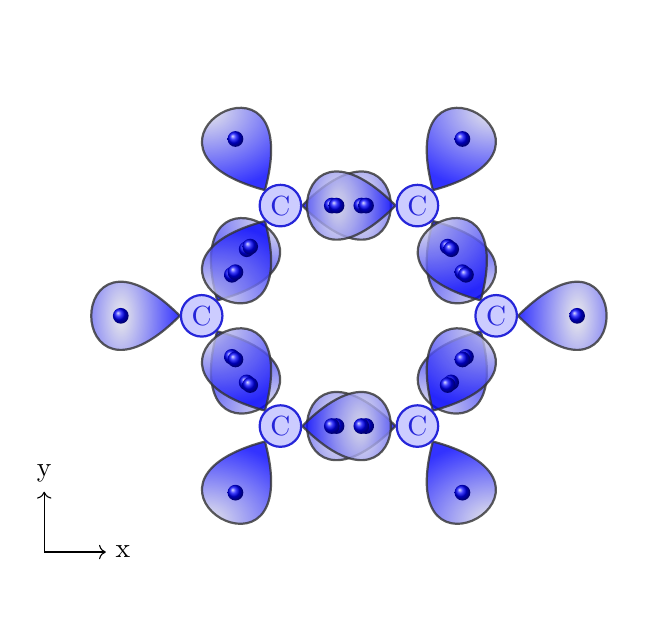
\begin{tikzpicture}
		    \node (x) at (-1,-3) {x};
		    \node (y) at (-2,-2) {y};
		    \draw[->] (-2,-3) -- (x);
		    \draw[->] (-2,-3) -- (y);
			\satom[name=C, color=blue, pos={(0,0)}]{
				blue/60/north east/2/1,
				blue/180/west/1,
				blue/300/south east/2/1
			}
			\satom[name=C, color=blue, pos={(1,1.4)}]{
				blue/0/east/2/1,
				blue/120/north west/1,
				blue/240/south west/2/1
			}
			\satom[name=C, color=blue, pos={(2.74,1.4)}]{
				blue/60/north east/1,
				blue/180/west/2/1,
				blue/300/south east/2/1
			}
			\satom[name=C, color=blue, pos={(3.74,0)}]{
				blue/0/east/1,
				blue/120/north west/2/1,
				blue/240/south west/2/1
			}
			\satom[name=C, color=blue, pos={(2.74,-1.4)}]{
				blue/60/north east/2/1,
				blue/180/west/2/1,
				blue/300/south east/1
			}
			\satom[name=C, color=blue, pos={(1,-1.4)}]{
				blue/0/east/2/1,
				blue/120/north west/2/1,
				blue/240/south west/1
			}
		\end{tikzpicture}}
	\caption{Carbon atoms in a hexagonal lattice are \(sp^2\) hybridised in the (\(x,y\))-plane.}\label{sp2}
    \end{subfigure}
    \caption{Benzene ring and its \(sp^2\) hybradised orbitals.}\label{Benz}
\end{figure}
This hybridisation lock all but one valence electron for the carbon atoms. These electrons exists in a p-orbital in the \(z\)-direction.
\cref{p} shows the valence orbitals of carbon.
\begin{figure}[H]
	\begin{center}
		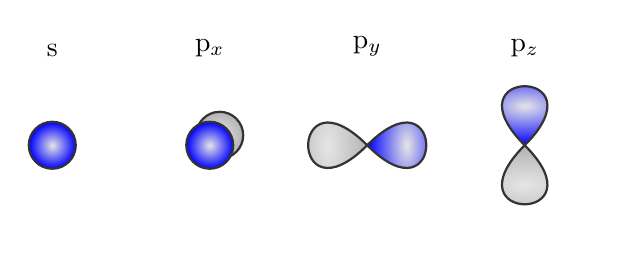
\begin{tikzpicture}
			\orbital[pos = {(0,3)}] {s}
			\node[above] at (0,4) {s};
			\orbital[pos = {(2,3)}]{px}
			\node[above] at (2,4) {p$_x$};
			\orbital[pos = {(4,3)}]{py}
			\node[above] at (4,4) {p$_y$};
			\orbital[pos = {(6,3)}]{pz}
			\node[above] at (6,4) {p$_z$};
		\end{tikzpicture}
		\caption{The valence orbitals of carbon.}
		\label{p}
	\end{center}
\end{figure}
The last electron in the p\(_z\) orbital does not mix with the tightly bound s, p\(_x\) and p\(_y\) electrons and moves freely. Thus these electrons have higher energies compared to the \(sp^2\) electrons and occupy states at the Fermi level. These electrons dominates transport in the graphene lattice. The p\(_z\) orbital is also known as the \(\pi\)-orbital and as such the electron lying there is called a \(\pi\)-electron. Through a carbon lattice the \(\pi\)-electrons will travel through \(\pi\)-orbitals. For a benzene ring the \(\pi\)-electrons at the highest occupied molecular state will travel through the p\(_\pi\)-orbitals switching sign as they travel as shown in \cref{sign}.
\begin{figure}[H]
	\begin{center}
		\pgfdeclarelayer{background}
		\pgfdeclarelayer{middle}
		\pgfdeclarelayer{foreground}
		\pgfsetlayers{background,middle,main,foreground}
		\begin{tikzpicture}
			\begin{pgfonlayer}{background}
				\orbital[pos = {(6,6)}]{-pz}
				\node[above] at (6,7) {-p$_\pi$};
				\orbital[pos = {(4,6)}]{pz}
				\node[above] at (4,7) {p$_\pi$};
				\draw[dashed, very thick] (6,6) -- (4,6);
				\draw[dashed, very thick] (7,4.73) -- (6,6);
				\draw[dashed, very thick] (4,6) -- (3,4.73);
			\end{pgfonlayer}
			\orbital[pos = {(7,4.73)}]{pz}
			\node[above] at (7,5.73) {p$_\pi$};
			\orbital[pos = {(3,4.73)}]{-pz}
			\node[above] at (3,5.73) {-p$_\pi$};
			\begin{pgfonlayer}{foreground}
				\orbital[pos = {(4,3.46)}]{pz}
				\node[above] at (4,4.46) {p$_\pi$};
				\orbital[pos = {(6,3.46)}]{-pz}
				\node[above] at (6,4.46) {-p$_\pi$};
				\draw[dashed, very thick] (4,3.46) -- (6,3.46);
			\end{pgfonlayer}
			\draw[dashed, very thick] (6,3.46) -- (7,4.73);
			\draw[dashed, very thick] (3,4.73) -- (4,3.46);
		\end{tikzpicture}
		\caption{When jumping from one carbon atom to another, the \(\pi\)-electron goes between p\(_\pi\)-orbitals. Such a jump is described by two matrix elements in the system's Hamiltonian.}
		\label{sign}
	\end{center}
\end{figure}
\subsection{Tight-binding}\label{tbtheory}
Now that the transport carrying electrons are defined the next step is describing the transport itself. For this purpose we employ the \textit{tight-binding} approximation. In this approximation the electrons are considered being tightly bound to the atoms. Contrary to a free electron gas approximation, the electrons does not spend time in between orbitals, but jump from orbital in atom \(a\) to orbital in atom \(b\). The Hamiltonian is represented as a matrix of hopping elements for a collection of neighbouring atomic orbitals, i.e. molecular orbitals, as well as the energy contained within each orbital (which will be addressed later on). This can be done by describing the orbitals as a Linear Combination of Atomic Orbitals (LCAO). The solution to the Schrödinger equation is then:
\begin{align}
	\Psi_{\mathrm{MO}} = \sum_{\alpha,R}c_{\alpha,R}\phi_{\alpha}(R)
\end{align}
where \(\phi_{\alpha}(R)\) is an atomic orbital at position \(R\), with \(\alpha\) denoting the valence of the orbital (\(2s,2p_x,2p_y,2p_z\)). In electron transport the states close to the Fermi level is of interest. These are namely the highest occupied molecular orbitals (HOMO), or the lowest unoccupied molecular orbitals (LUMO). As stated earlier only the \(\pi\)-electrons is then of interest.
The electrons' motion can be described with the hopping matrix of elements:
\begin{align}
	V_{pp\pi} = \bra{\phi_{\pi}(1)}\hat{H}\ket{\phi_{\pi}(2)}\label{V}
\end{align}
Physically this means that there is a potential between the \(\pi\) orbitals of neighbouring atoms \(1\) and \(2\). In our tight-binding approximation we consider only hop between nearest neighbours. The element
\begin{align}
	\epsilon_0 = \bra{\phi_{\pi}(1)}\hat{H}\ket{\phi_{\pi}(1)}
\end{align}
is the average energy of the electron on atom \(1\) and, it is common to define the hopping energy relative to this, i.e. \(\epsilon_0 = 0\).
If the atoms or their environment differs, so does the on-site potential.\newline
\cref{benzex} contains an illuminating example of how the tight-binding approximation can be used to describe simple carbon systems.
\section{Hamiltonian for periodic systems}\label{hamilsec}
%!TEX root = ../Main.tex
 In the following sections, the focus will be to present and explain how to calculate band structures, local density of states and transmission, through \textit{python}-programming, using Tight Binding approximation for any periodic structure. For simplicity, all initial examples and calculations will be done on a simple system, to make sure the different steps are easy to follow. The system can be seen in \cref{pointplot}.
\subsection{Creating the on-site Hamiltonian and hopping matrices}
The first and most essential parts needed for calculations is the \textit{on-site} Hamiltonian \(\mathbf{h_0}\) and the \textit{hopping} matrices \(\mathbf{V},\ \mathbf{V}^{\dagger}\). The starting point is a matrix, containing set of coordinates \(x_0,y_0,z_0\), representing atom positions  and a set of unit vectors \(\mathbf{u}_x, \ \mathbf{u}_y, \ \mathbf{u}_z\). The unit vectors will be the basis of the unit cell containing all atom coordinates. From now on, only the x and y coordinates will be considered as graphene is considered purely a 2D material.
\begin{figure}[h]
	\centering
	\begin{subfigure}[b]{0.45\textwidth}
		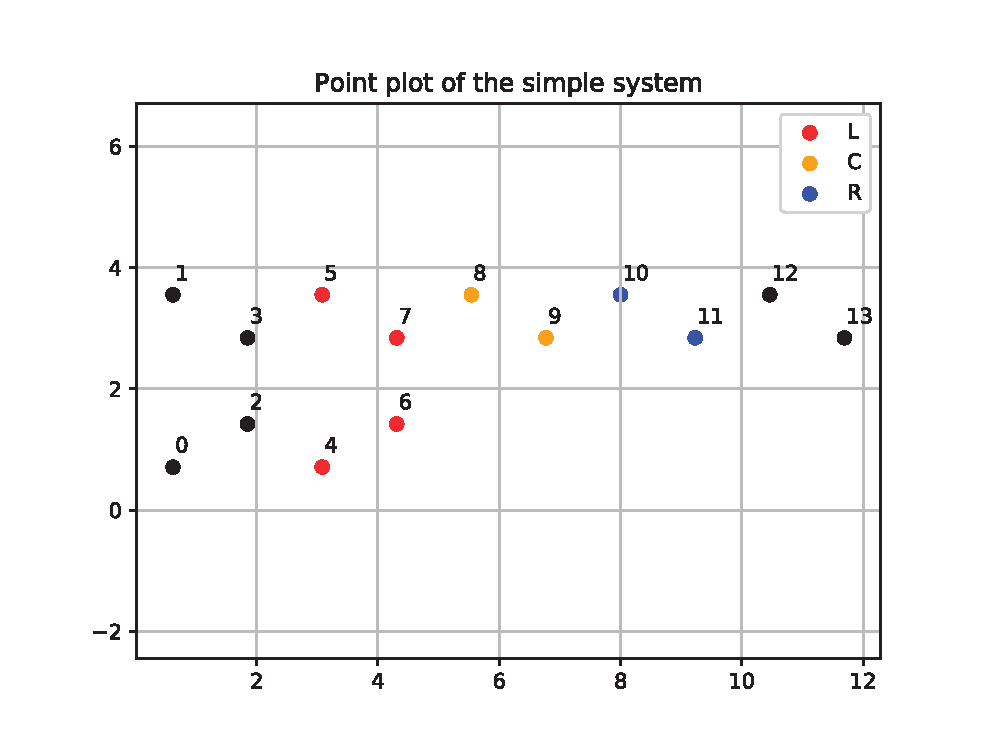
\includegraphics[width=\textwidth]{Figures/pointplot.eps}
		\caption{Figure showing the simple system. Every atom in the unit cell has an index, here from 0 to 7. The blue and red colours mark the left and right contacts of the system.}
		\label{pointplot}
	\end{subfigure}
	~ %add desired spacing between images, e. g. ~, \quad, \qquad, \hfill etc.
	%(or a blank line to force the subfigure onto a new line)
	\begin{subfigure}[b]{0.45\textwidth}
		\includegraphics[width=0.7\textwidth]{Figures/BetaBandstructures.eps}
		\caption{Figure showing the band structure of the simple system.}
		\label{bandssimple}
	\end{subfigure}
	\vskip\baselineskip %add desired spacing between images, e. g. ~, \quad, \qquad, \hfill etc.
	%(or a blank line to force the subfigure onto a new line)
	\begin{subfigure}[b]{0.45\textwidth}
		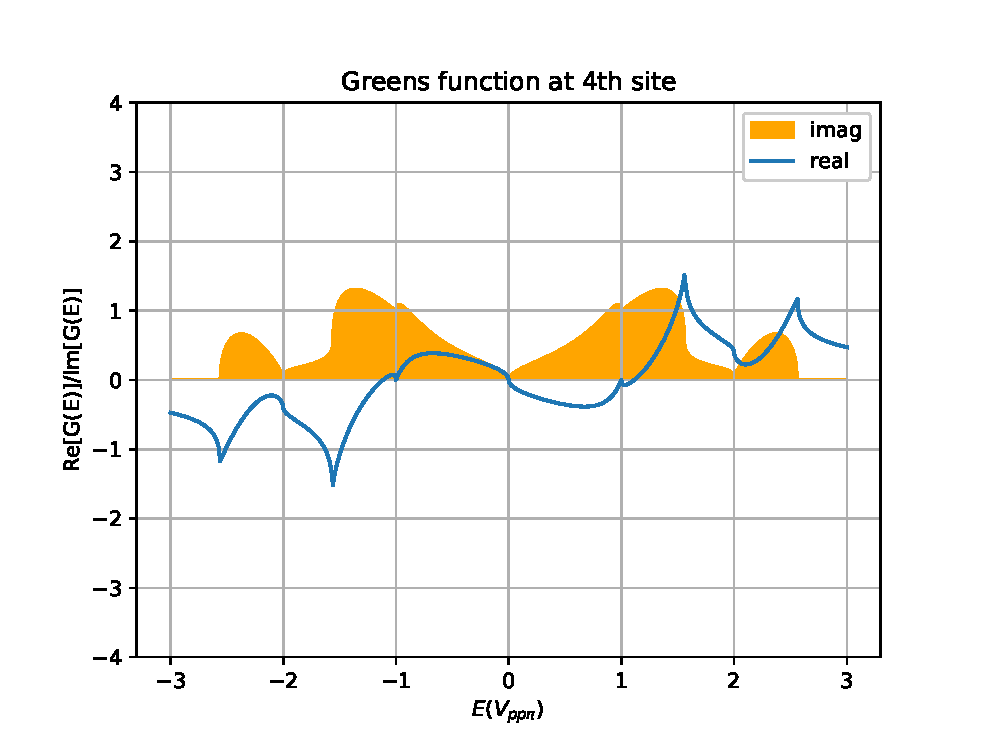
\includegraphics[width=\textwidth]{Figures/BetaimrealTE.eps}
		\caption{A plot showing the real and imaginary part of Green's function at the zeroth site resulting from the recursion routine on the simple system. Note that the yellow imaginary part is the representation of the local density of states.}
		\label{LDOSsimple}
	\end{subfigure}
	~
	\begin{subfigure}[b]{0.45\textwidth}
		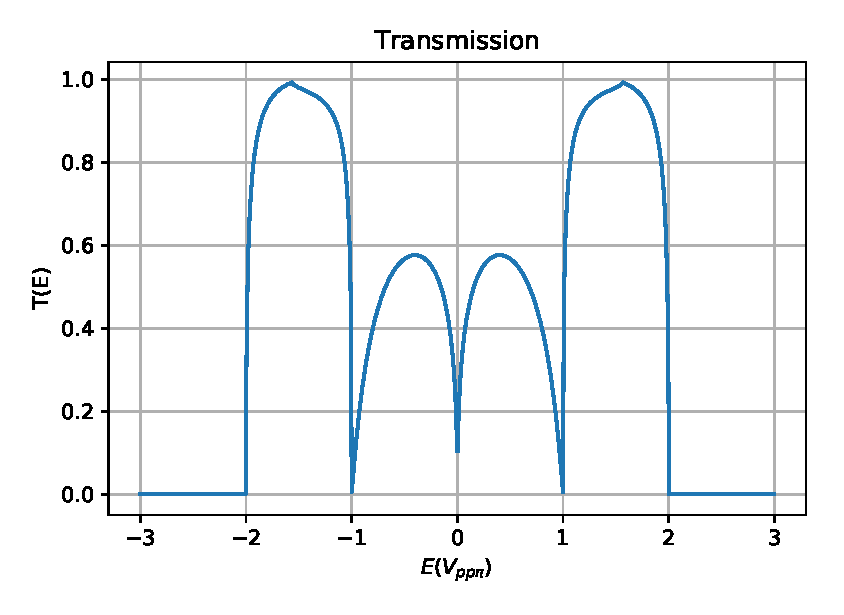
\includegraphics[width=\textwidth]{Figures/BetaTE.eps}
		\caption{\vspace{-4\baseFigure showing the resulting transmission through the simple system}
		\label{Transsimple}
	\end{subfigure}
	\caption{Figure of the different calculations executed on the simple system, using the developed scripts. }\label{eksamplefigure}
\end{figure}
The on-site Hamiltonian represents the interaction of atoms within the unit cell and the hopping matrices represents the interaction of atoms between periodically repeated unit cells. 
In \cref{atomrepfig} a visual representation of NPG with periodically repeated unit cells can be seen. For the rest of the report, the on-site Hamiltonian will all ways be the centre cell while the hopping matrices will be the cells surrounding the on-site Hamiltonian (See \cref{repfig} for a generalised visual representation of the concept). \\
In practice, the scenario is that only a data set of coordinates given from scratch. The first step is to get the on-site Hamiltonian. As mentioned the on-site Hamiltonian represents the interaction of atoms within the unit cell. The approach is then to find the atoms which interact. The interaction is based on the inter-atomic distance between atoms, so naturally one wants to find the distance between all atoms in the unit cell. To do this a subtraction of all possible combinations of two sets of atom coordinates must be done. Then taking the norm of all individual results to get the distance. A function called \textit{Onsite} have been developed to do just this. In \cref{npouter} the function can be seen.
\im{Listings/Functions.py}{31}{38}. 
\vspace{-1\baselineskip}
\captionof{listing}{The outer operator in numpy is manifested as two nested loops. On lines xx-xx each atomic distance is calculated. Line xx replaces all nearest neighbour distances with an input potential, leaving the rest as zero. Lastly the diagonal is subtracted from the matrix.\label{npouter}}\vspace{\baselineskip}
The function produces a matrix which contain all distances between all atoms in the unit cell. The Tight Binding model dictates that only atoms with a specific inter-atomic distance interact. Therefore the function has implemented a threshold (\cref{npouter} line xx) to determine whether a given distance is too great for interaction or small enough for interaction. All distances above the threshold will be changed to a 0-element in the on-site Hamiltonian matrix, representing zero interaction and all distances below the threshold will be changed to 1 to represent interaction between atoms. Finally The on-site Hamiltonian is multiplied with a on-site potential (scalar). The on-site potential \(V_{pp\pi}\) differs depending on the system. Now the on-site Hamiltonian is complete and the product is a matrix containing 0's and 1's to represent interaction between atoms in a unit cell. \\
Moving on to the hopping matrices one first has to realise that the interactions are happening in a 2D plane. This has to be kept in mind when describing interaction between unit cells repeated in all directions in the plane. Effectively this means that six hopping matrices should be created. One in the x-direction, one in the y-direction, one in the xy-direction and their hermitian conjugates. Graphically this corresponds to a structure of this kind:
\begin{figure}[H]
	\centering
	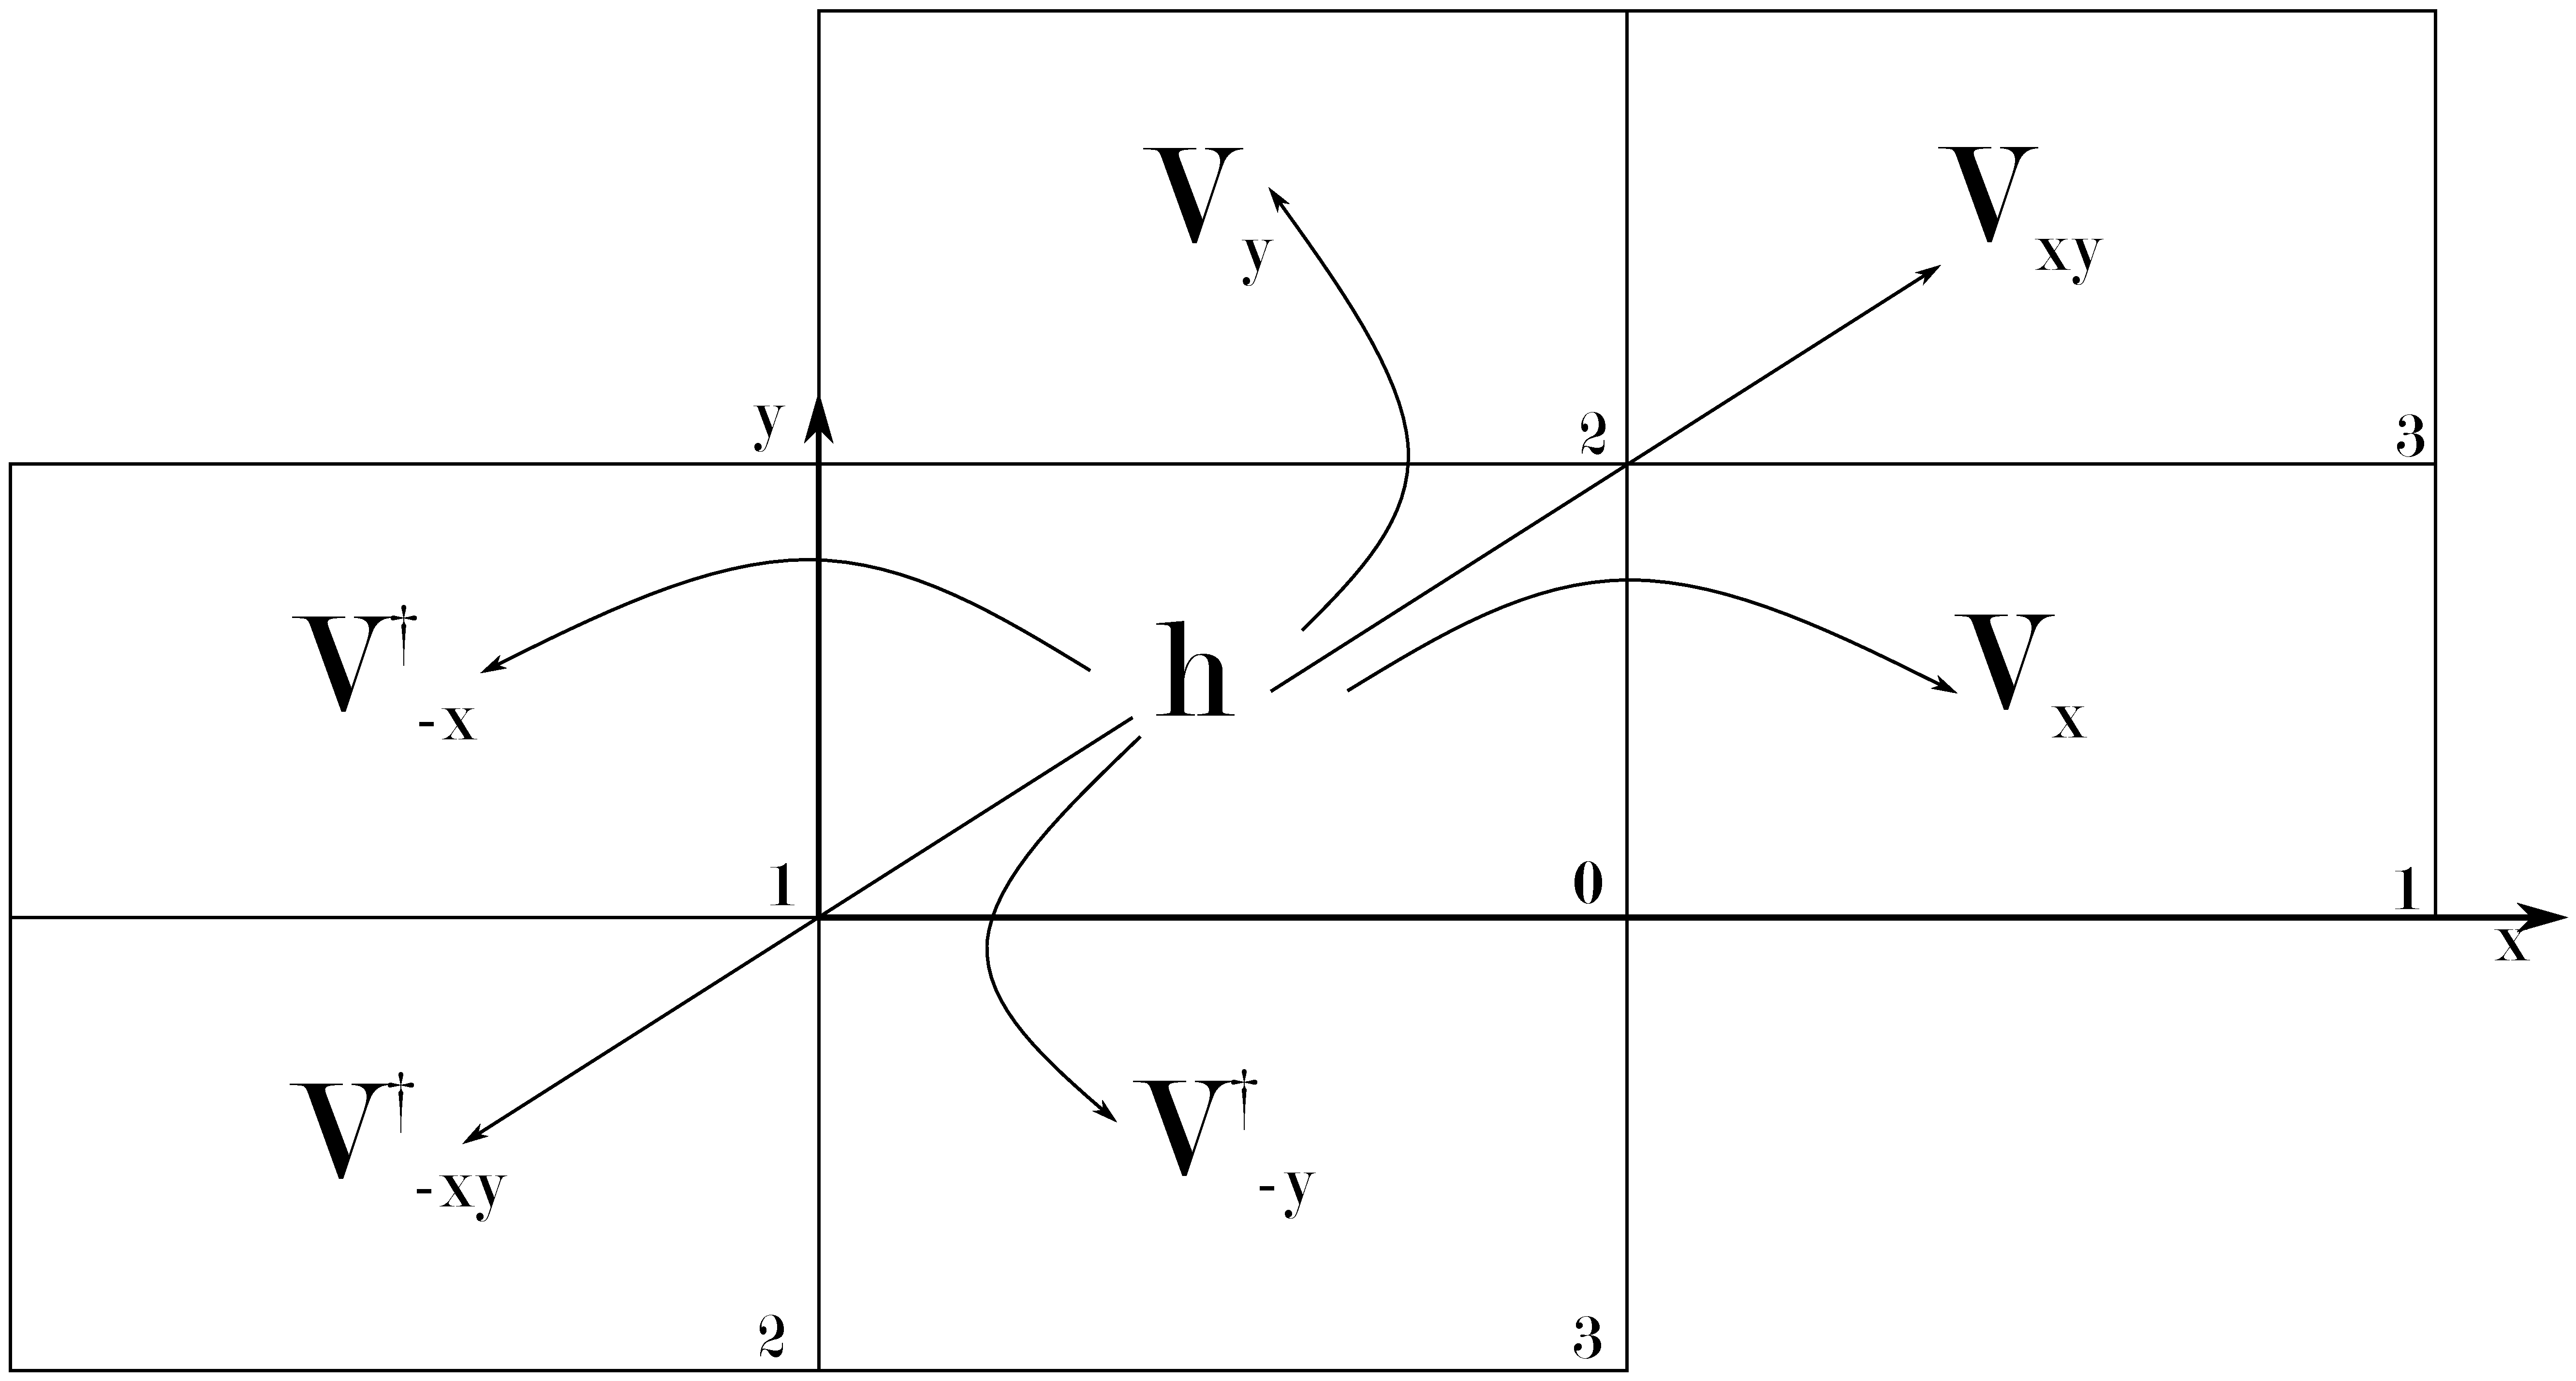
\includegraphics[width = 0.7\textwidth]{Figures/repfig.eps}
	\caption{Representative figure of how the on-site Hamiltonian along with its hopping matrices are structured}
	\label{repfig}
\end{figure}
In practice this is done by shifting the original \(x_0,y_0\) coordinates by the given unit vectors \(\mathbf{u}_x,\mathbf{u}_y\). By addition of the unit vectors to the original coordinate matrix one can get three new coordinate matrices \(\mathbf{xy}_{shift-x}=x_0,y_0 + \mathbf{u}_x\), \(\mathbf{xy}_{shift-y}=x_0,y_0 + \mathbf{u}_y\) and \(\mathbf{xy}_{shift-xy}=x_0,y_0 + \mathbf{u}_x+\mathbf{u}_y\). With these three matrices what follows is basically the same method used to get the on-site Hamiltonian. The only difference being that it will be distances between atoms in the on-site Hamiltonian and the shifted matrices respectively. That way it is the distance, and thus the interaction, between the on-site Hamiltonian and the repeated unit cells that is calculated. The three resulting hopping matrices are denoted \(\vb{V}_{1x}\), \(\vb{V}_{2y}\) and \(\vb{V}_{3xy}\). They represent interaction (hopping) in the "forward" direction (left-to-right) (See \cref{repfig}). To create the hopping matrices hopping in the "backwards" (right-to-left) direction (See \cref{repfig}) one simply has to transpose the hopping matrices. These matrices are denoted with a dagger: \(\vb{V}_{1x}^{\dagger}\), \(\vb{V}_{2y}^{\dagger}\) and \(\vb{V}_{3xy}^{\dagger}\). The matrices are programmed using the developed function \textit{Hop}, which can be seen in \cref{appfigs}, \cref{hopfunc}. To show how the on-site Hamiltonian and the hopping matrices look, see \cref{matrixmap} for a figure of the resulting matrix-maps from calculation on the small simple system. It has been stitched together like in \cref{repfig}. To see how the function running the calculation for the hopping matrices look in \cref{appfigs}, \cref{hopfunc}. 
\begin{figure}[H]
	\centering
	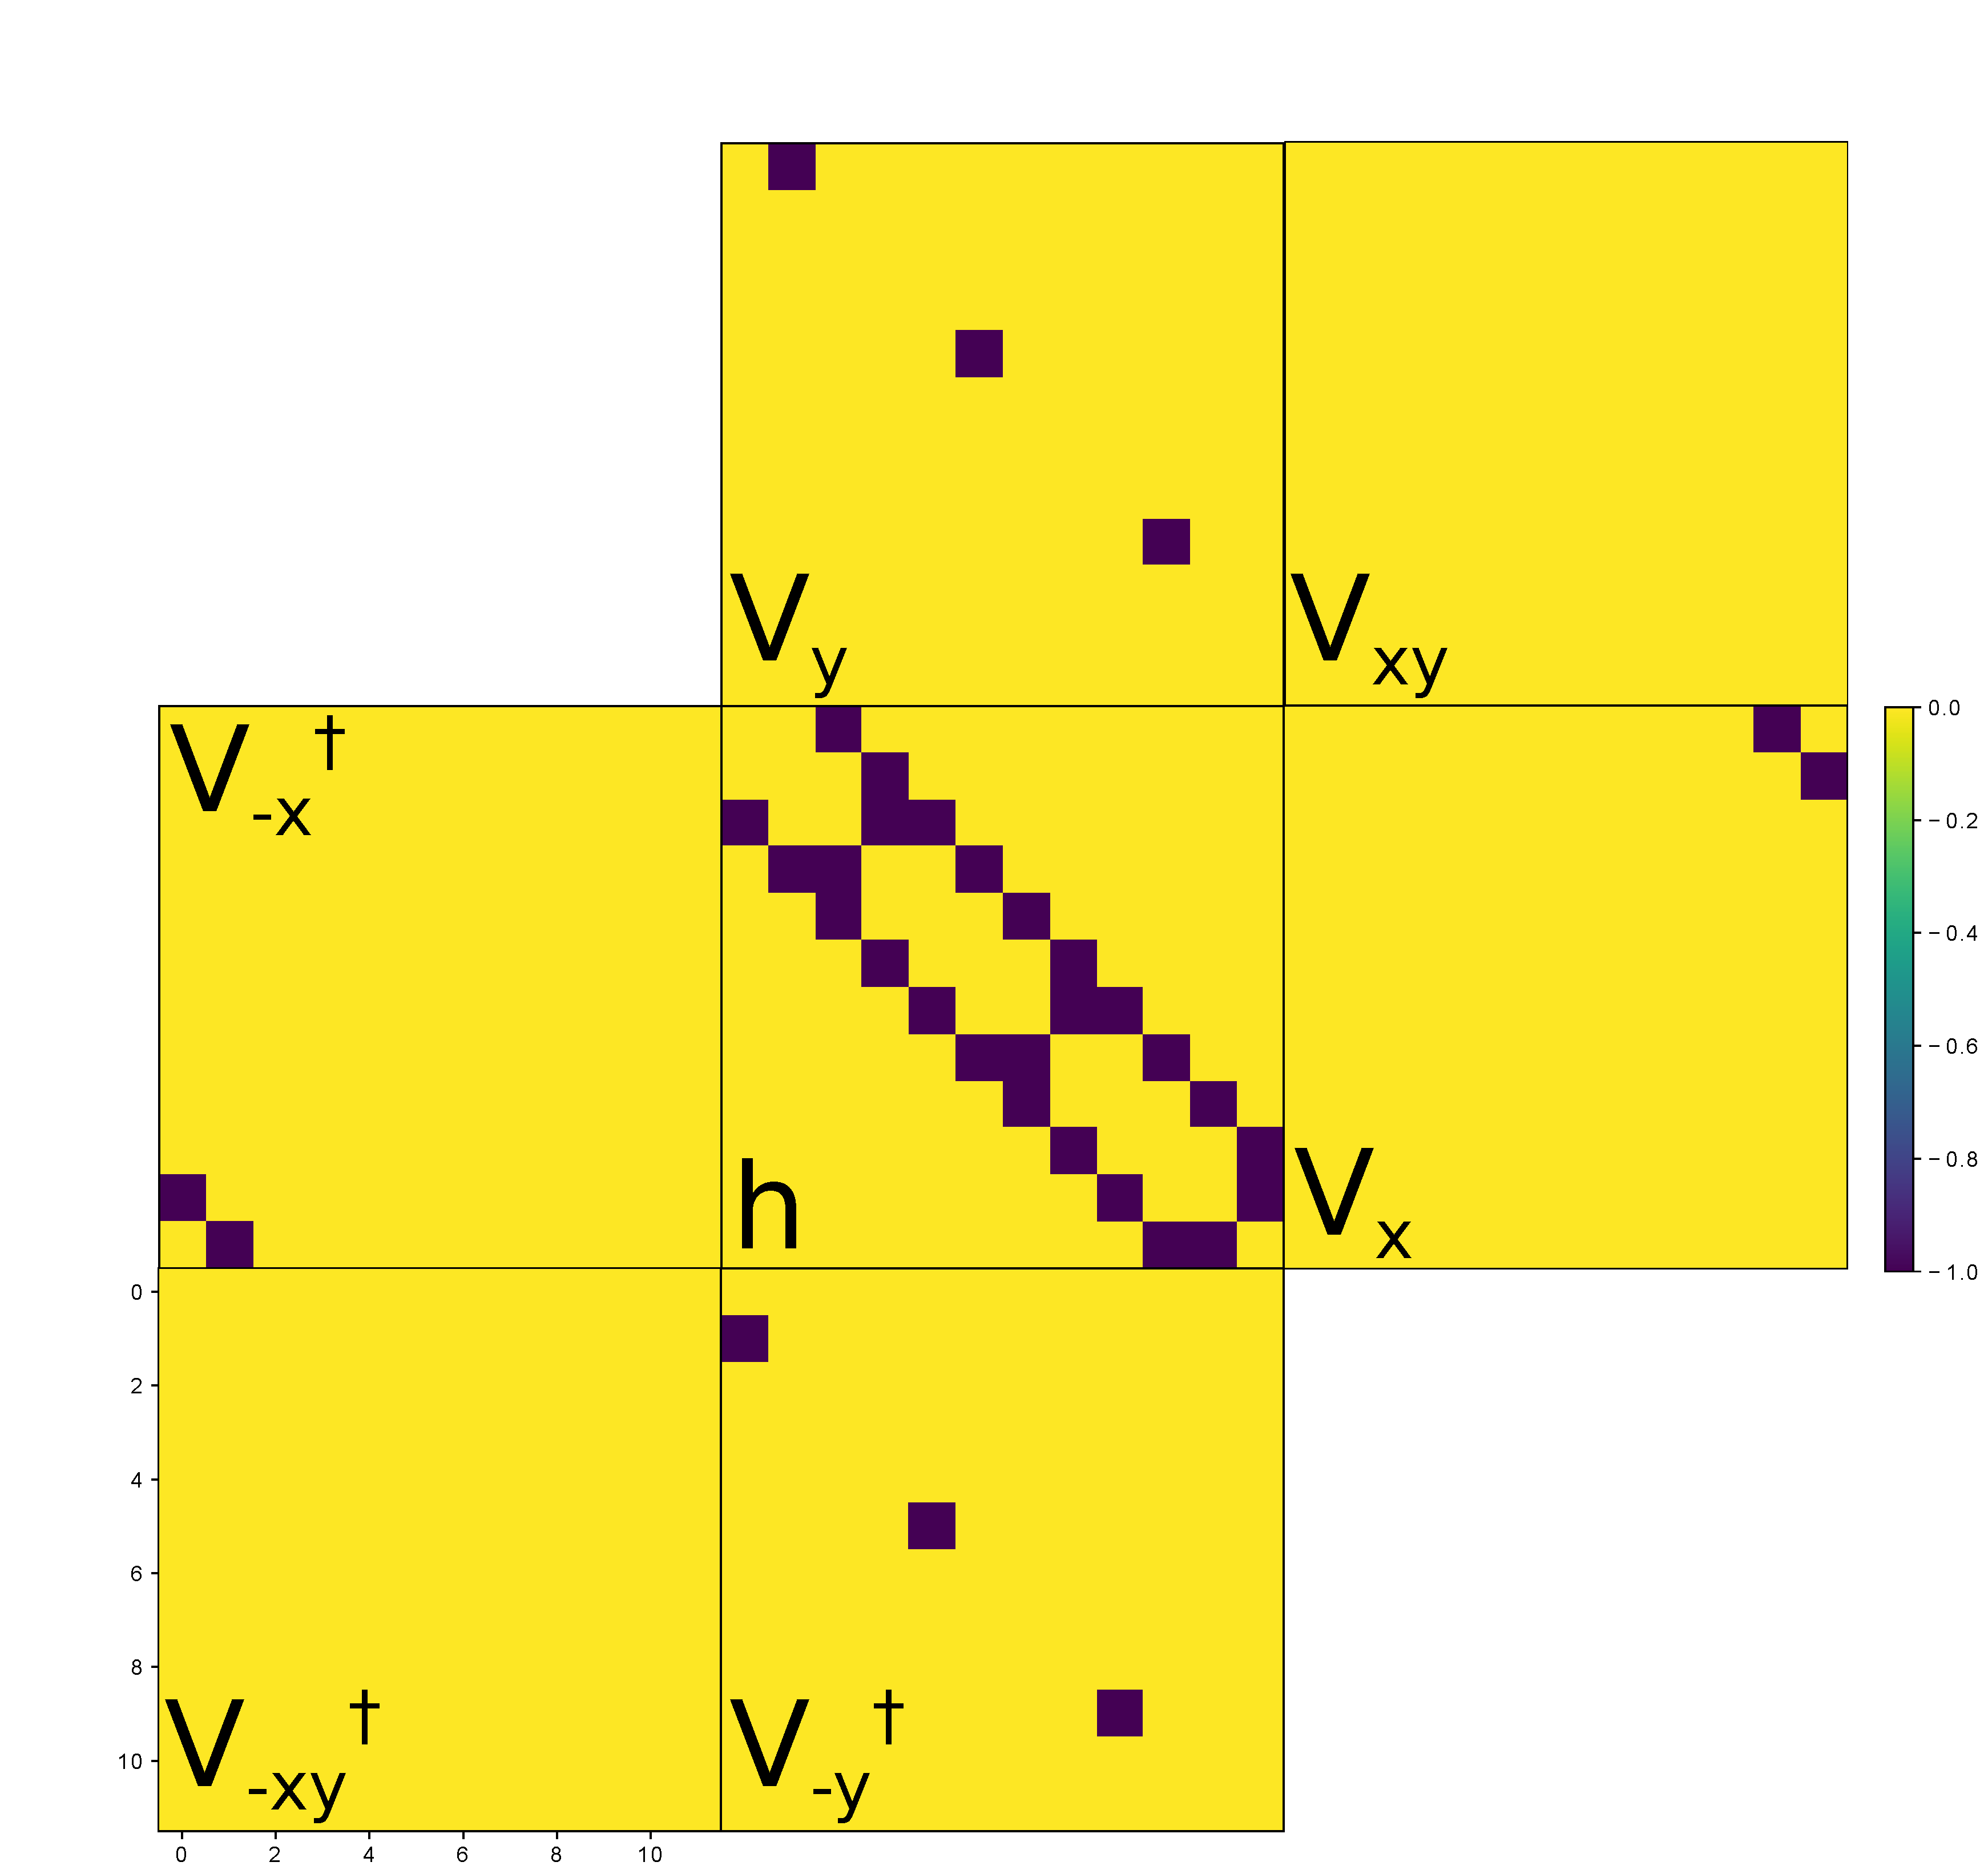
\includegraphics[width=0.7\textwidth]{Figures/stitch.eps}
	\caption{Matrix maps from calculation on an arbitrary graphene system with a unit cell of 12 atoms. The on-site Hamiltonian along with all its hopping matrices are stitched together like in figure \cref{repfig}. All the dark spots represent a hopping of an electron to its nearest neighbour i.e. a 1 element and yellow represents a 0 element}
	\label{matrixmap}
\end{figure}
\subsection{Defining the full Hamiltonian and solving the Schr\"{o}dinger equation}\label{FullHam}
Now that the on-site Hamiltonian along with its hopping matrices have been created, the next step is to create the full Hamiltonian in order to solve the Schr\"{o}dinger equation for the system as a whole. This is an eigen-value/vector problem. The Schr\"{o}dinger equation needs to be solved to get the eigen energies for the system as they will be used to produce band structure plots later on. In essence the full Hamiltonian denoted \(\vb{H}\) is a sum of the on-site Hamiltonian and its corresponding hopping matrices multiplied by a complex exponential function that has the appropriate phase relative to the hopping matrix:\begin{align}\label{hamileq}
	\vb{H}(k_x,k_y) = \vb{h}_0 & + (\vb{V}_{1x}e^{-ik_x} + \vb{V}_{1x}^{\dagger}e^{ik_x}                              \\ \nonumber
	                           & + \vb{V}_{2y}e^{-ik_y} + \vb{V}_{2y}^{\dagger}e^{ik_y}                              \\
	                           & + \vb{V}_{3xy}e^{-ik_x}e^{-ik_y} + \vb{V}_{3xy}^{\dagger}e^{ik_x}e^{ik_y}) \nonumber
\end{align}Here \(k\) represents a continuous variable between 0 and \(\pi\) along the \(\dfrac{1}{x}\)- and \(\dfrac{1}{y}\)-axis in reciprocal space.
Using the full Hamiltonian, the Schrodinger equation can be solved
\begin{align}
	\vb{H}(k_x,k_y)\vb*{\phi}_{k} = \vb*{\epsilon}_n (k_x,k_y) \vb*{\phi}_k
\end{align}
Where \(\vb*{\phi}_k\) is the and \(\vb*{\epsilon}(k_x,k_y)\) is the eigen energies. \\
In practice this is done by defining a function, here called \textit{Hkay}, that takes the on-site Hamiltonian, the hopping matrices, and \(k_{x/y}\) as inputs and outputs the eigenvalues, using numpy's \textit{numpy.linalg.eigh}. The number of eigenvalues in the output corresponds to the dimension of the full Hamiltonian. In \cref{fullhamil} the code for the function is shown.
\im{Listings/Functions.py}{50}{59}
\vspace{-1\baselineskip}
\captionof{listing}{Function producing the full hamiltonian, corresponding to \cref{hamileq} the inputs x and y corresponds to the \(k_x\),\(k_y\) .\label{fullhamil}}\vspace{\baselineskip}
\subsection{Producing band structures}
%An important intrinsic information in any solid state matter is of course the band structure as it gives information about allowed electron energies at different points in the material. Specifically for NPG, the band structure may be used to track the changes of electronic transport upon changing the bridges connecting GNR's within NPG.
In order to calculate and visualise the band structure of the simple system, one need to define the full Hamiltonian \(\mathbf{H}\) in two directions. When working with band structures and periodic systems it is common to note points in space with respect to the \textit{Brillouin Zone} which is a primitive cell in reciprocal space. Therefor 
a continuous variable \(k\) is introduced. it extends in two directions in (\(-k_{x}\)) and (\(k_{y}\)), which correspond to lengths between the symmetry points \(X\), \(\Gamma\) and \(Y\) in the Brillouin zone. Here \(\Gamma\) is the origin \((0,0)\). Practically this corresponds to making two plots, one for each pair of symmetry points. The y-values in each plot correspond to the eigenvalues obtained by the \textit{Hkay} function described in \cref{FullHam}. The number of eigen energies, and effectively the number of bands in the plot is dictated by the dimension of the Hamiltonian. \(n\times n\)-matrix \(\rightarrow\) \textit{n} eigen energies (bands). However plots produced in this report will only show a few of these bands in a small energy range. In the case of the simple system, the full Hamiltonian for obtaining the eigen energies that corresponds to directions \(X\) and \(Y\) are:\begin{align}
	X: \ \vb{H}_{X} = \vb{h}_0 + (\vb{V}_{1x}e^{ik_x} + \vb{V}_{1x}^{\dagger}e^{-ik_x} + \vb{V}_{2y} + \vb{V}_{2y}^{\dagger} + \vb{V}_{3xy}e^{ik_x} + \vb{V}_{3xy}^{\dagger}e^{-ik_x}) \\
	Y: \ \vb{H}_{Y} = \vb{h}_0 + (\vb{V}_{1x} + \vb{V}_{1x}^{\dagger} + \vb{V}_{2y}e^{-ik_y} + \vb{V}_{2y}^{\dagger}e^{ik_y} + \vb{V}_{3xy}e^{-ik_y} + \vb{V}_{3xy}^{\dagger}e^{ik_y})
\end{align}Using the eigenvalues as y-values in the two plots, putting the two plots together will yield a final plot of the band structure shown in \cref{bandssimple}. 



\section{Greens Functions, Self Energy and the Recursion Routine}\label{greensec}
%!TEX root = ../Main.tex
The Green's function and self energies play the central role when it comes to obtaining the LDOS as well as electron transport in a system. In fact, the imaginary part of the Green's function is the LDOS for a specific site in a system. What the Green's function and self energy actually is and how they come about will here be explained formally, to motivate the practical use in the following sections.\subsection{Green's functions and self-energy}\label{greensandself}
Some of the concepts in this section will be explained using  the simle system as an example (\cref{atomrepfig}). However, in the following section (\cref{recursionroutinesec}) the focus will revert back to the simple system from \cref{pointplot}. \begin{figure}[H]
	\centering
	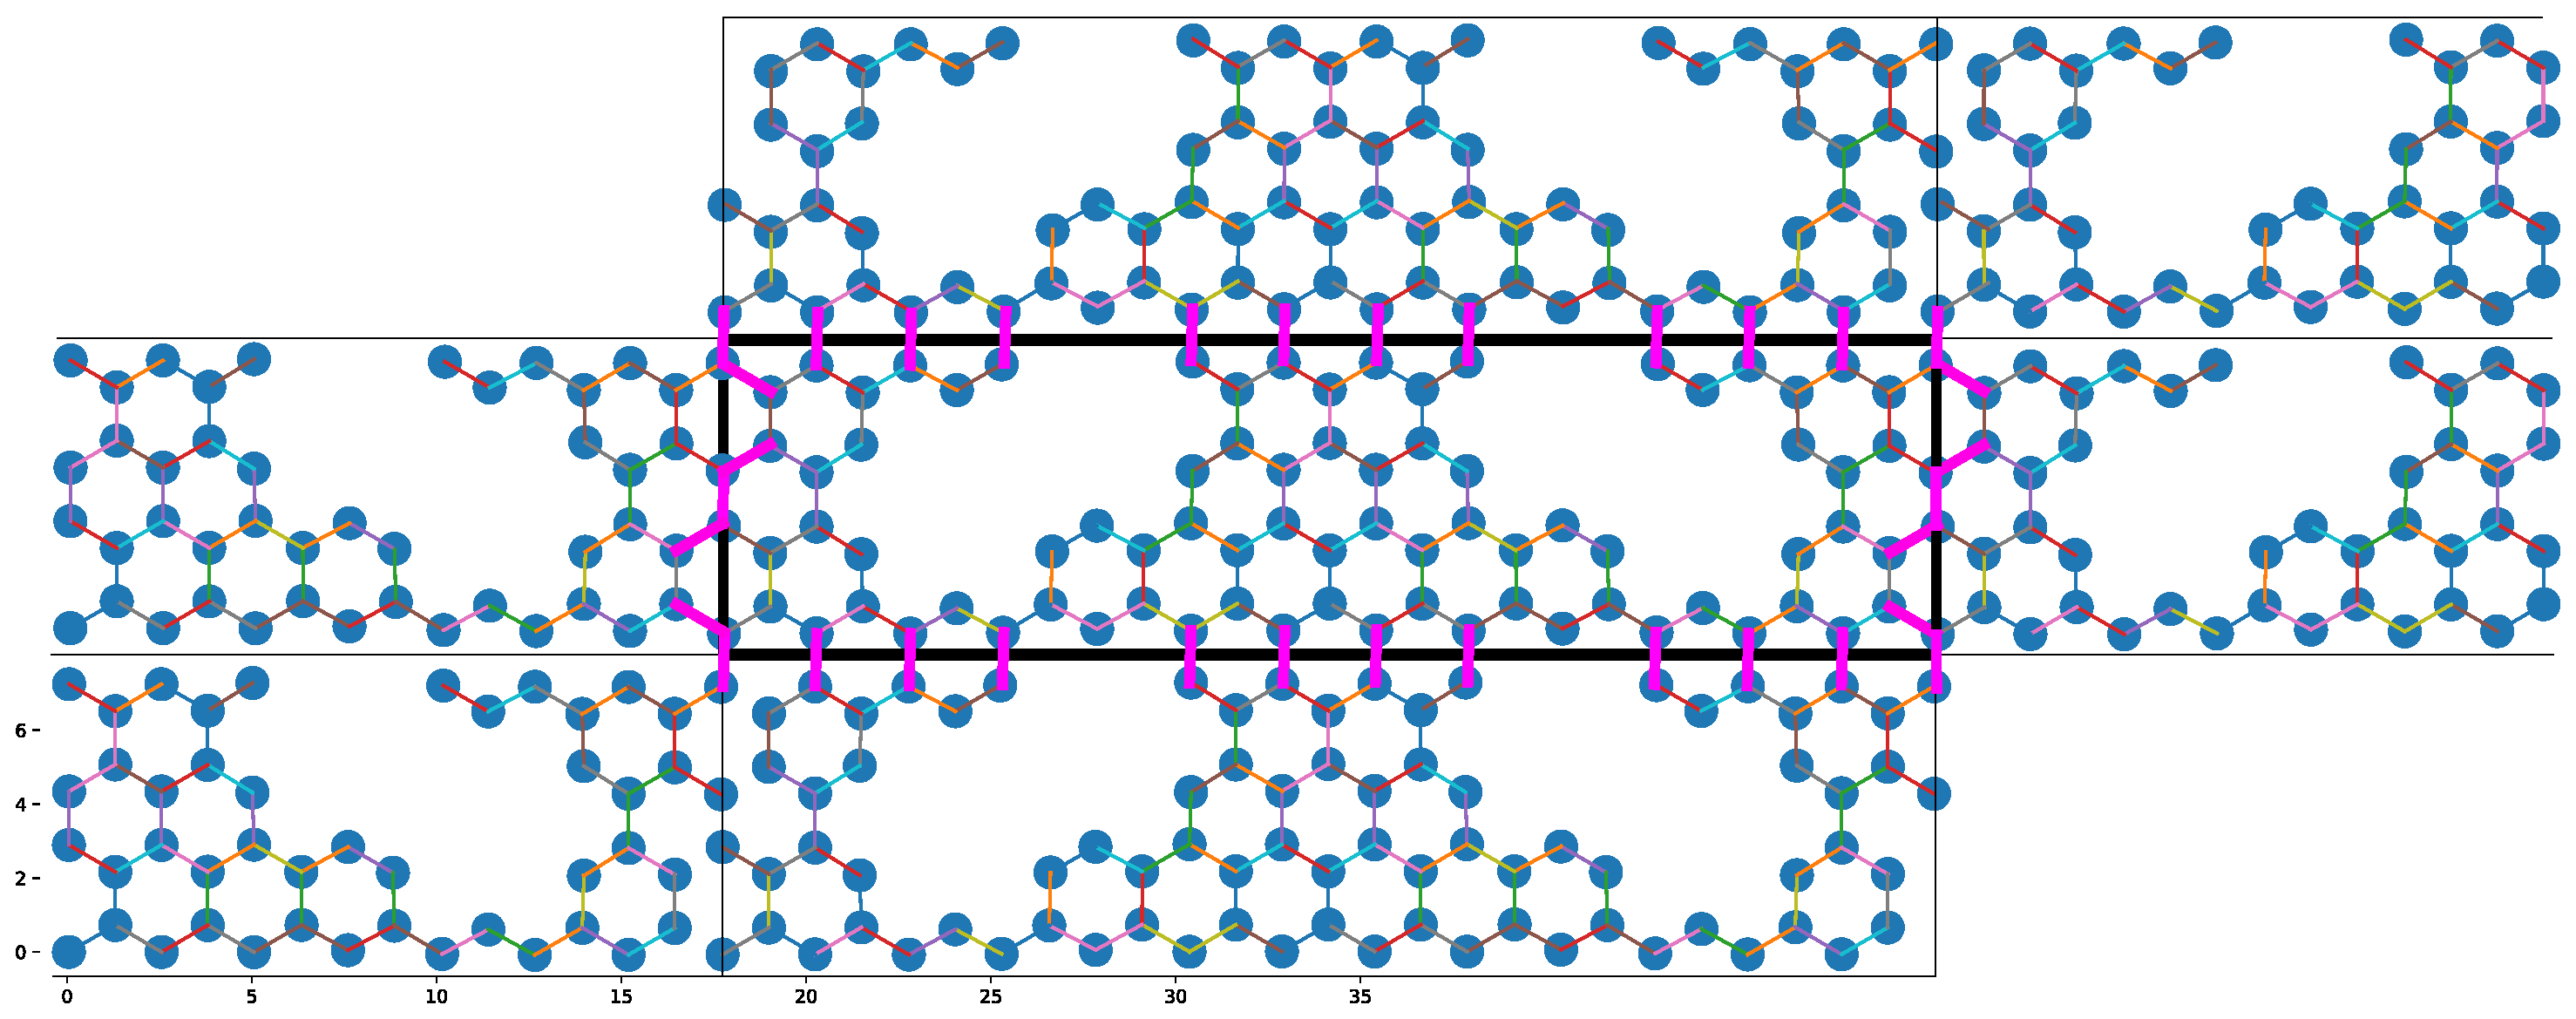
\includegraphics[width=\textwidth]{Figures/representativestructure2.eps}
	\caption{Visual representation of the periodic NPG-structure. The atoms surrounded by the black box in the centre represents the unit cell. The neighbouring boxes are unit cells repeated periodically. Note that the two cells left and right with respect to the centre cell has been cut in half for figure space. The pink lines crossing the black box represents the link between the nearest neighbours in the adjacent cell.}
	\label{atomrepfig}
\end{figure}
%\begin{align}
%\mathbf{H}\phi(t) &= i\pdv{t}\phi(t) \\
%\mathbf{H}\mathbf{G}(t) &= i\pdv{t}\mathbf{G}(t)
%\end{align}
%with specific boundary conditions, namely\begin{align}\label{boundary}
%    \phi(t=0) = f
%\end{align}
%The Green's function has the additional property that \(\mathbf{G}(t=0)=\mathbf{1}\) which means the one can solve the TDSE for any initial value of \(t\)  if one has solved the equation for the Green's function first.\begin{align}\label{greenssolution}
%    \phi(t)=\mathbf{G}(t)f
%\end{align}
%From \cref{greenssolution} it can be seen that the Green's function propagates the value \(f\) at \(t=0\). Now, if the Hamiltonian is time independent one can also consider time independent solutions to the Schr\"{o}dinger Equation. All states will then be oscillating with the same complex phase, at a specific energy \(E\). This will be given by \(e^{-iEt}\).
Imagine a system like the one in \cref{atomrepfig}. It contains a unit cell in the centre, marked by a black border, surrounded by repeated unit cells in all directions. The aim is to explain how electrons move through this region. Suppose all cells surrounding the centre cell are considered "contacts" in the sense that they represent a semi-infinite chain of molecules and that they are the source of electrons (or states) that is injected in to the centre cell. What the Green's function is doing is that it "takes the states through" the centre region. It propagates the states in this particular area. In other words, the Green's function is the solution to the Schr\"{o}dinger Equation in this area and the equation has the form
\begin{align}\label{Greensunsolved}
	[(E+i\eta)\mathbf{1}-\mathbf{H}]\mathbf{G}(E) = \mathbf{1}
\end{align}
From this equation one can also get the Green's function as
\begin{align}\label{Greenssolved}
	\mathbf{G}(E) & = \mathbf{1}([(E+i\eta)\mathbf{1}-\mathbf{H}])^{-1} \\
	              & = [(E+i\eta)\mathbf{1}-\mathbf{H}]^{-1}
\end{align}
The Green's functions in these equations are represented as matrices that contain all the individual Green's functions for the unit cell as well a the Green's functions for the rest of the chain. As seen in the equations, all that is needed to get the Green's function for a unit cell, in theory, is an energy and the Hamiltonian of the unit cell. Note that the solution to the Green's function matrix is a diagonal matrix with the two first off diagonals. This is because of rules for nearest neighbour interaction dictated by the Tight Binding approximation. As the Green's functions for all unit cells in a potentially semi-infinite system are needed, in practice, one has to turn to more sophisticated methods to obtain all the Green's functions, namely recursion. More on that shortly. For now this is the introduction to the Green's function. How it relates to a unit cell in a system and that it is the source of the LDOS in a unit cell.\\
As described  one can use the Green's functions to get the propagation of states through a specific on-site Hamiltonian. However, if the system contains a range of cells, possibly infinitely many, the Hamiltonian would be of infinite size and the inversion in \cref{Greenssolved} would be impossible to do practically. The solution to this, is to model a semi-infinite tight binding chain of atom/molecules and then use \textit{recursion} on this chain. The way the recursion is done is to remove every second cell in the chain. Because the chain is semi-infinite, the yield would just be a new semi-infinite chain. Continuing this way the system can be reduced to a finite size which can actually be worked on. Say one continues to remove every second element in the chain, then in the end, the cells would be too far apart to interact an no hopping between cells would occur. At this point the recursion should stop. More on how this is done practically later.  For now one just have to keep in mind that the removing cells in the chain effectively changes to coupling between them and this is where \textit{self energy} comes in. The self energy is what describes the effective coupling between a cell and the rest of the semi-infinite chain. And it can be derived by looking at a cell at the very end of the semi-infinite chain and see how it couples to the rest. First one needs the Green's functions. The Green's matrix for this single cell would be given by the equation in \cref{Greenssolved}. This is before when only one cell and thus one matrix had to be considered. But now, there is an semi-infinite amount of cells and an semi-infinite amount of matrices to consider. However, the cell in the end of the chain only interacts with the cell next to it and so on. Considering this one can write op an equation equivalent to that of \cref{Greensunsolved} but as system of matrix equations for the chain.
\begin{align}\label{Greenssystem}
	\begin{pmatrix}
		z\mathbf{1}-\mathbf{H}_c & -\mathbf{V}^{\dagger} \\ -\mathbf{V} & (z-\varepsilon')\mathbf{1}
	\end{pmatrix}
	\begin{pmatrix}
		\mathbf{X}      & \mathbf{G}_{0c} \\
		\mathbf{G}_{c0} & \mathbf{G}_{00}
	\end{pmatrix}
	=
	\begin{pmatrix}
		\mathbf{1} & \mathbf{0} \\
		\mathbf{0} & \mathbf{1}
	\end{pmatrix}
\end{align}
where \(\varepsilon'\) is the on-site Hamiltonian of the first cell, \(z\) is \(E+i\eta\),  \(\mathbf{G}_{0c/c0}\) is the Green's matrices coupling the cell to the rest of the chain and \(\mathbf{X}\) is the Green's matrices for the rest of the chain. This is also assuming one knows the Green's function within the chain \(\mathbf{G}_c\) and that the chain has constant hopping and on-site elements \(\mathbf{H}_c,\mathbf{V},\mathbf{V}^{\dagger}\).
Solving this system for \(\mathbf{G}_{00}\) and eliminating \(\mathbf{G}_{0c}\), which is unknown, one gets
\begin{align}\label{greenszero}
	\mathbf{G}_{00}(z) = (z-\varepsilon'-\Sigma(z))^{-1}
\end{align}
where \(\Sigma(z)\) is the self-energy. One can isolate the self energy from the equations above to
\begin{align}
	\mathbf{\Sigma}(z) = \mathbf{V}[z\mathbf{1}-\mathbf{H}_c]^{-1}\mathbf{V}^{\dagger}
\end{align}
And this concludes the formal introduction to Green's functions and self energy.\subsection{Obtaining first cell self-energy and Green's matrix through programming}\label{recursionroutinesec}
For simplicity and in order to check whether the routine would yield the expected results, the system in \cref{pointplot} is use as an example. The goal is to get the Green's functions for the centre unit cell in the semi-infinite chain and the self energies coupling to rest of the chain right and left. Specifically for the simple system one should imagine first having one centre unit cell like \cref{pointplot} and then repeating it infinitely in the left and right direction. The fact that there is a left \textit{and} right self energy is that the unit cell lies within the semi-infinite chain and not at the very end as described in \cref{greensandself}. To be assured, this does not conflict with any of the preciously mentioned formalism and the left and right self energies are quite easily obtained as one shall see shortly. As mentioned the goal is to get the Green's functions of a specific unit cell and the self energies related to it. If the Green's matrix \(\mathbf{G}\) represents the whole chain, then the equation of the whole system would be equivalent to that of \cref{Greensunsolved}. Considering the Green's functions for specific unit cell in question, it would correspond to one column in the system of equations, say the first. One can define the on-site Hamiltonian \(\mathbf{h}_0\) for the specific unit cell and its hopping matrices \(\mathbf{V},\mathbf{V}^{\dagger}\).  The two hopping matrices correspond to hopping left or right in the chain respectively. These can be obtained using the functions already developed in \cref{hamilsec}. Throughout this section they will be named \(a_0 = \mathbf{V}^{\dagger}, \ b_0 = \mathbf{V}, \ e_{s0} = \mathbf{h}_{s}\). The recursion is an iterative process and so the zero index indicates the starting point of the iterations and the \textit{s} index indicates that it is the Hamiltonian of the specific wanted cell. One can also define a Green's function for a single unit cell as \(g_0 = (z-e_{0})^{-1}\) just like \cref{Greensunsolved} where \(e_{0}=\mathbf{h}\) which is the on-site Hamiltonian of the other cells. With these elements a system of equations, similar to \cref{Greensunsolved} can be setup. The first difference being that the identity matrix is replaced by its first column, because the solution of interest is that one first column in the Green's matrix. The second is that the first element in the Hamiltonian matrix \(\mathbf{H}\) is related to the specific single unit cell \(\mathbf{h}_s\). Next a range of multiplications of the different elements stated so far will be shown, and afterwards it will be explained how these affect the system of equations to give recursion. The multiplications are:
\begin{align}
	a_1    & = a_0 \times g_0 \times a_0                  \nonumber                      \\
	b_1    & = b_0\times g_0\times b_0                   \nonumber                       \\
	e_1    & = e_0 + a_0\times g_0\times b_0 + b_0\times g_0\times a_0 \label{matmulrec} \\
	e_{1s} & = e1_{0s} + a_0\times g_0\times b_0          \nonumber                      \\
	g_1    & = (z - e_1)^{-1} \nonumber
\end{align}
These equations constitutes the first iteration in the recursion and they can be repeated indefinitely. In the matrix system of equations  these multiplications effectively shifts all elements in the matrix by one column and because the matrix is diagonal, it will leave the first column of the matrix empty. The column can then be removed and this is exactly what corresponds to removing a cell in the semi-infinite chain. Keeping on doing these multiplications, raising the index by +1 every time, one can move through reduce the system as a whole removing of columns (cells) in the system of equations. In the end one will obtain re-normalised Hamiltonians and hopping matrices which is then used to get the Green's functions and self energies through these simple equations:
\begin{align}
	\mathbf{\Sigma}_R & = e_s - h                   \nonumber       \\
	\mathbf{\Sigma}_L & = e - h - \mathbf{\Sigma}_R \label{outputs} \\
	\mathbf{G00}      & = (z - e_s)^{-1} \nonumber
\end{align}
Programming this recursion is fairly simple as all which is needed is a while loop which iterates over the equations in \cref{matmulrec} until a threshold has been reached. The threshold is determined by the value of the hopping matrix \(a_0\). As it reaches a value close to zero, there is no longer any effective interacting (hopping) between the cells because of removal of cells and the recursion should stop.
In \cref{recurfunc} the code for the routine is shown. Line xx-xx is the listing of elements before iteration, xx-xx is the while loop with the equations from \cref{matmulrec}. Note that some intermediate multiplications are made f.ex. \textit{ag = a0 @ b0}. This is for run-time optimisation only. In  line xx-xx the iteration indexed 0 gets redifned so that it corresponds to the most recent iteration. Finally in xx-xx the definition of the outputs as per \cref{outputs} is stated.\im{Listings/Functions.py}{62}{89}
\vspace{-1\baselineskip}
\captionof{listing}{The while loop in the recursion routine. The matrix elements are overwritten with the new variables until the resulting matrix is small enough to diagonalise\label{recurfunc}}\vspace{\baselineskip}
This concludes how recursion works and how the first cell Green's function as well as the self-energies is obtained.
\subsection{Plotting the real and imaginary part of the first cell Green's function}
One of the results possible to obtain via the recursion routine is the Green's function of the centre unit cell in relation to the rest of the chain. As mentioned the imaginary part of the elements Green's matrix is the LDOS of the different sites in the unit cell. With a relatively simple approach, the Green's matrix elements can be obtained as a function of energy, using a \textit{for loop}, looping over a range of energies which is then used as input in the \textit{RecursionRoutine} function (\cref{recurfunc}), see \cref{plotcode}:
\im{Listings/SelfEnergyByRecursion.py}{64}{68}
\vspace{-1\baselineskip}
\captionof{listing}{Code showing the loop which produces the complex Green's function (or y) values for a range of energies used in the plot.\label{plotcode}}\vspace{\baselineskip}
This gives information about the LDOS at a specific energy and place in space, namely a specific atom in the unit cell. The resulting plot for the simple system (atom index 4) can be seen in \cref{LDOSsimple}. As seen in the plot... Note that the plot only represents the LDOS for a specific site on the molecule and that they may change radically from site to site (see \cref{appfigs}, \cref{siteLDOSplot} for an example using the same system as \cref{pointplot}). The site can be changed by choosing another index in \cref{plotcode} line 68, which corresponds to the atom indices in \cref{pointplot}.

\section{Transmission Routine}\label{transec}
%!TEX root = ../Main.tex
The conclusion of the preliminary work revolves around the Transmission Routine. Here all the functions producing on-site Hamiltonians, full Hamiltonians, hopping matrices, band structures, self energy and Green's functions by recursion play their part in getting the transmission through the material. \textit{This part is an attempt to describe the basic theory behind transmission/transport and it is very likely to need rework, additions and editing} The transmission tells us the probability whether an electron will be transported trough all the possible \(\pi\)-orbitals in a "device region" at different energies and thus how the "device region" affects the overall current through larger systems. This means that the system will have to be well defined before one can use the functions developed for calculation of the different parts needed for production of transmission. The "device region" contains at least one central unit cell as well as a "left" and "right" unit cell. The left and right unit cell represents the contact region of the device i.e. the two parts that connects to the "rest" of the system/molecule. It is assumed that the "rest of the molecule" represent a system that is made up of unit cells which can be reduced by recursion, though not necessarily identical on each side (left and right). Knowing which "blocks" the system contains and how to obtain them with the already developed functions, three main ingredients are needed to obtain the transmission through a device. The first one is the Green's function for the device region \(\mathbf{G}_D\). The device region of cause includes the device Hamiltonian \(\mathbf{H}_D\) and in addition, \(\mathbf{H}_D\) contfor which one needs the device Hamiltonian \(\mathbf{H}_D\) as well as the left and right selfenergies \(\mathbf{\Sigma}_L, \ \mathbf{\Sigma}_R\). The left and right selfenergies constitutes the second ingredient and can be obtained through left and right hopping matrices as well as the left and right on-site Green's functions. The last main ingredient are \(\mathbf{\Gamma}_L,\ \mathbf{\Gamma}_R\) which are matrix operators describing the coupling between the left and right parts of Hilbert space. They are called rate equations because..... The rate equation are obtained via the self energies in the following fashion: 
\begin{align}\label{rateeq}
\mathbf{\Gamma}_{L/R} = i(\mathbf{\Sigma}_{L/R} - \mathbf{\Sigma}^{\dagger}_{L/R})
\end{align}To give an overview of how the different matrices are defined in relation to a system an illustration has been made. See \cref{systemillu}. Using the Green's function, left/right self energies as well as the left/right rate matrices, the transmission, as a function of energy, can be obtained via the following equation:
\begin{align}
    T(E) = \text{Tr}[\mathbf{\Gamma}_R\mathbf{G}_D\mathbf{\Gamma}_L\mathbf{G}_D^{\dagger}](E)
    \label{transeq}
\end{align}
Where Tr is the trace of the matrix product. 
\begin{figure}
    \centering
    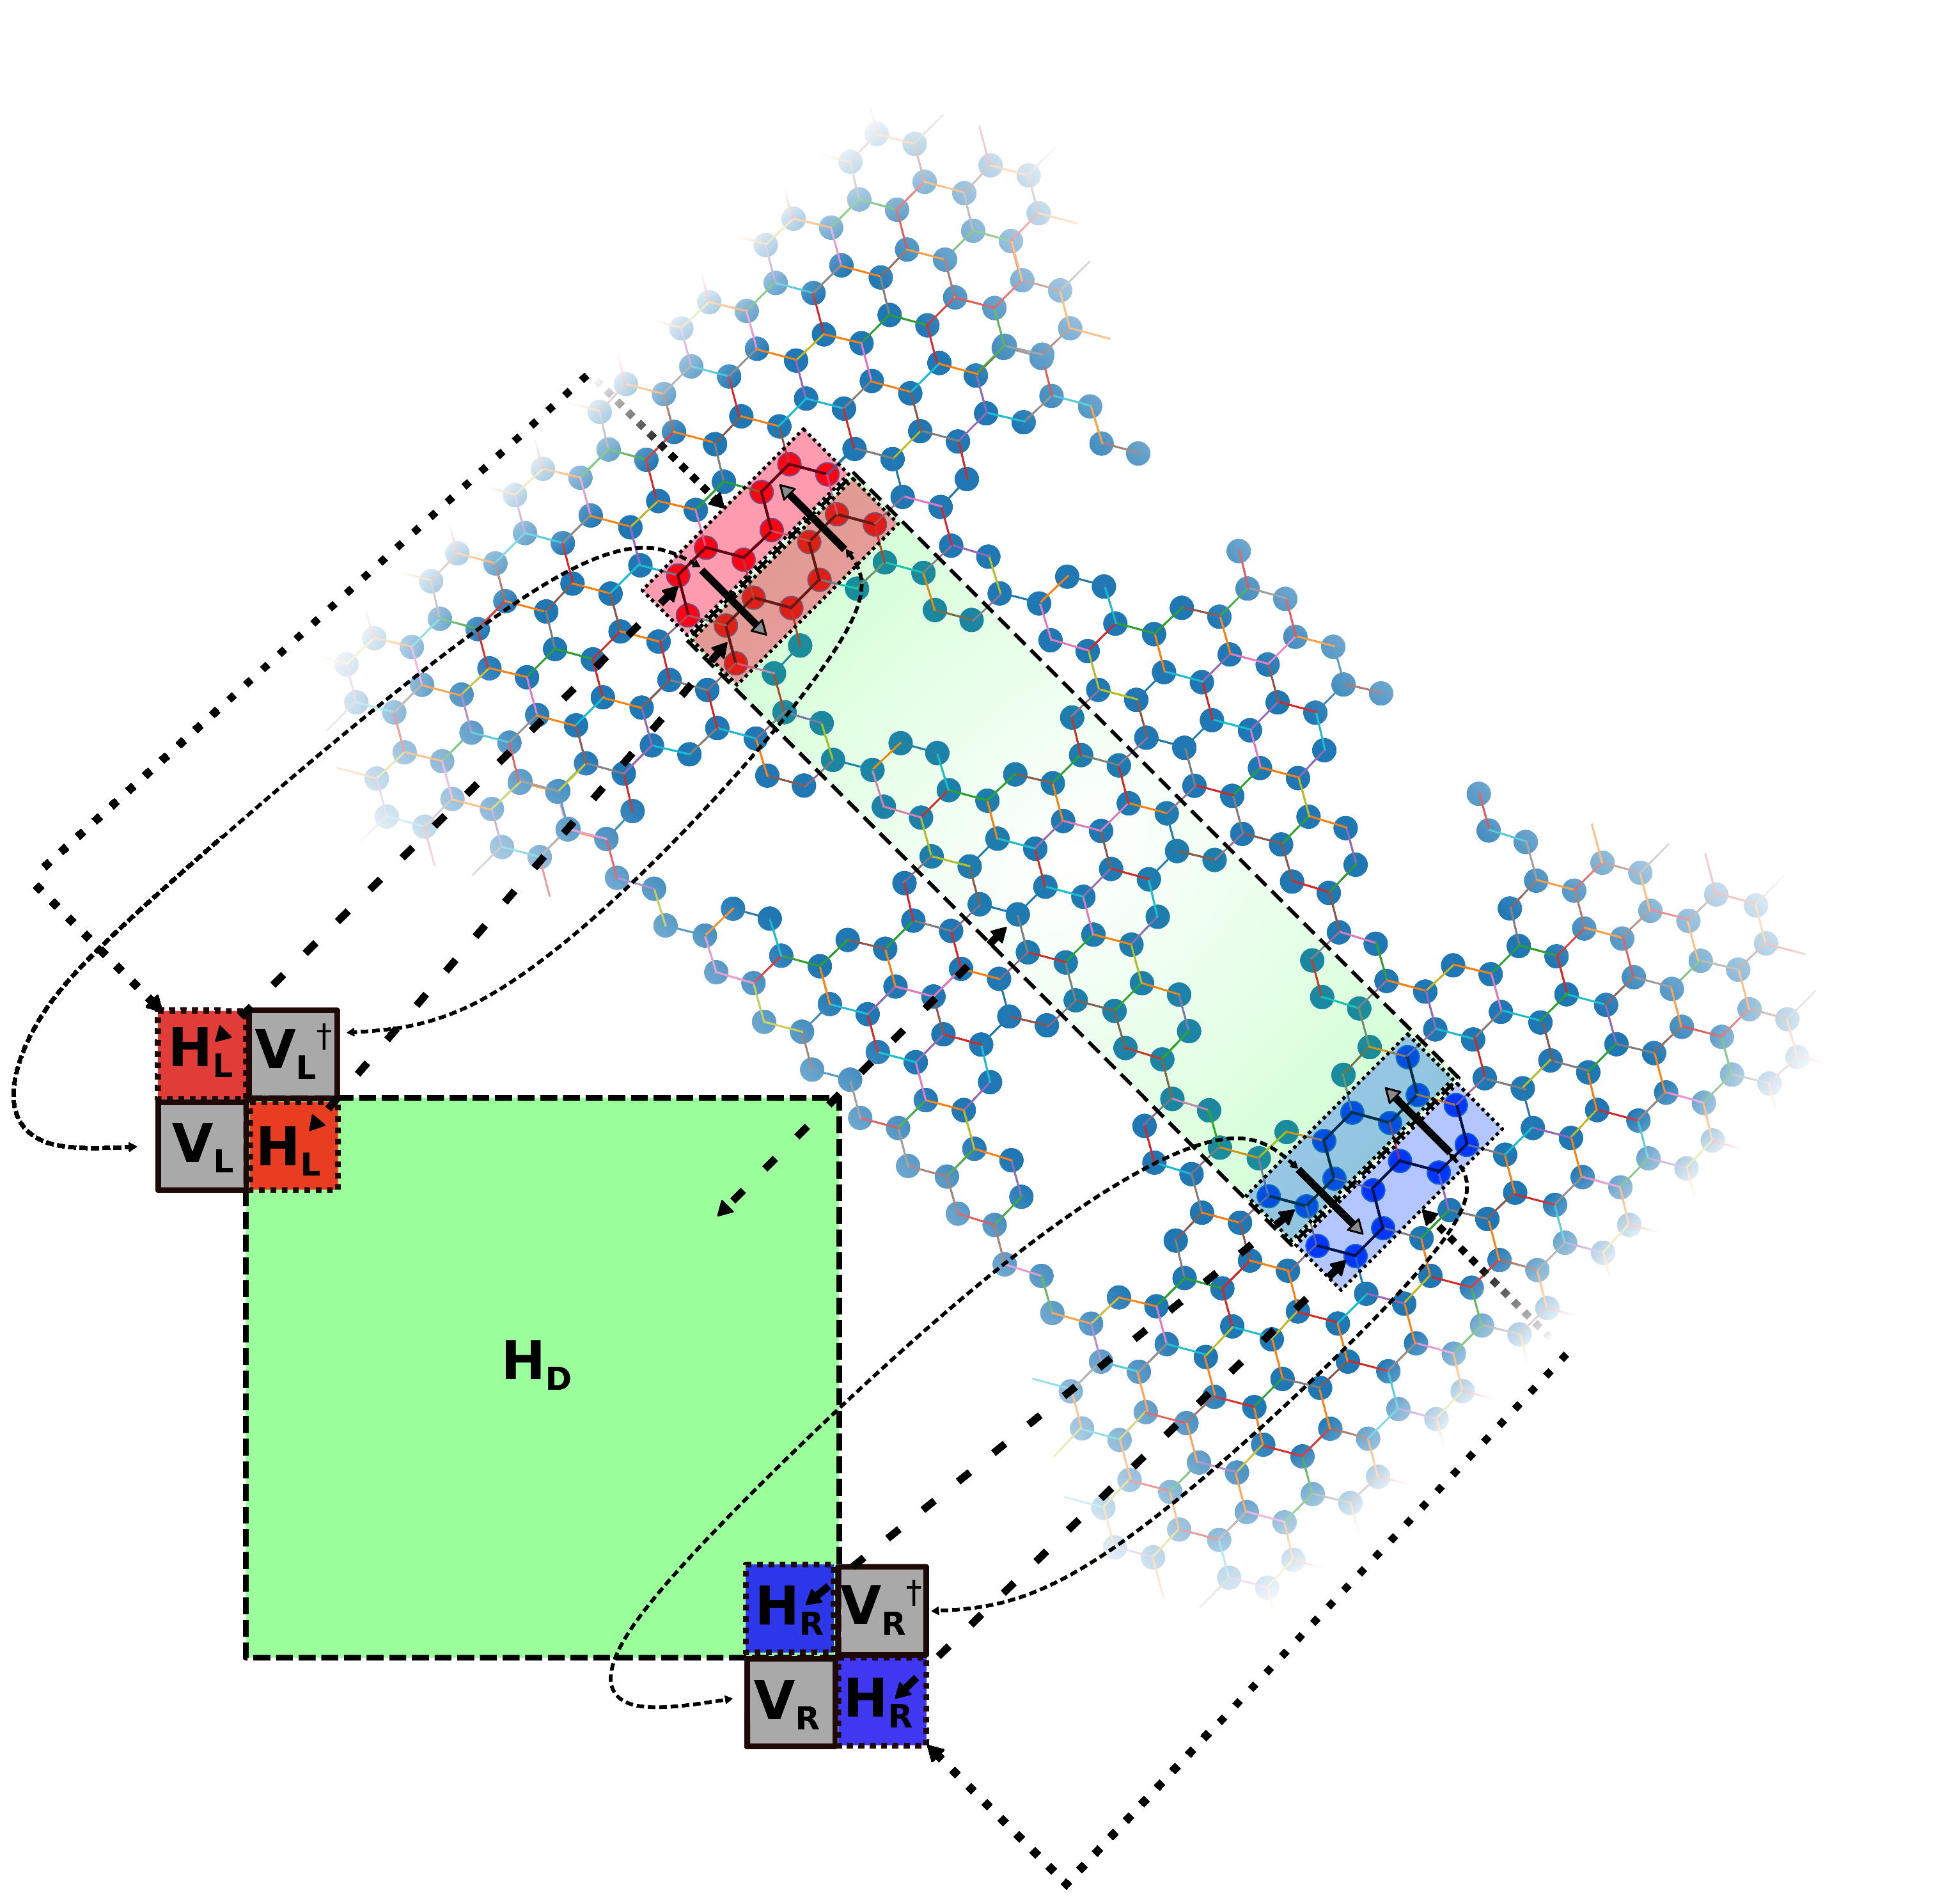
\includegraphics[width=0.9\textwidth]{Figures/illu.eps}
    \caption{Illustration showing how the different parts of the system are translated into matrix blocks. On the graphene the green box is the unit cell of the device. It includes one red and blue box which themselves are unit cells of the left and right contacts. These unit cells can be translated into Hamiltonian matrices \(\textbf{H}_D, \ \textbf{H}_L,\ \textbf{H}_R\) as illustrated. Note that because the first of the left and right unit cells (red and blue) are inside the device (green region), they can be picked out of \(\textbf{H}_D\) directly and so it is not necessary to make them from scratch. The two other unit cells lying outside the device region represents what could be an infinite contact region. The contact region is therefore potentially of an infinitely bigger dimension compared to the device region, however, by recursion, this region can be collapsed into a single Hamiltonian of same dimension as the one inside the device region. Finally the two fat black arrows (not dotted) on each side of the device represents the hopping between the device and contact region. Note that the direction of hopping corresponds to a specific hopping matrix. F.ex. left-to-right is the ordinary hopping matrix while right-to-left is its conjugate (for both left and right side of the device).}
    \label{systemillu}
\end{figure}
\subsubsection{Transmission in 1D a simple example}
As with the Recursion Routine, the development of this routine will be build up around a small system in order to make sure that the obtained results are as expected, thereafter generalising the routine to suit all kinds and sizes of system. First thing is to define the device in the same manner as \cref{systemillu} so that the device Hamiltonian \(\textbf{H}_D\) can be obtained through the already defined function \textit{Onsite}. The left and right Hamiltonian \(\textbf{H}_{L/R}\) are thus picked out as described in \cref{systemillu}. A smart function has been implemented in order to allow the user to choose the left and right contact cells using indices given to each atom in the system of choice (See \cref{basicstructurewithcontacts} for an example).
\begin{figure}
\begin{subfigure}[b]{0.4\textwidth}
		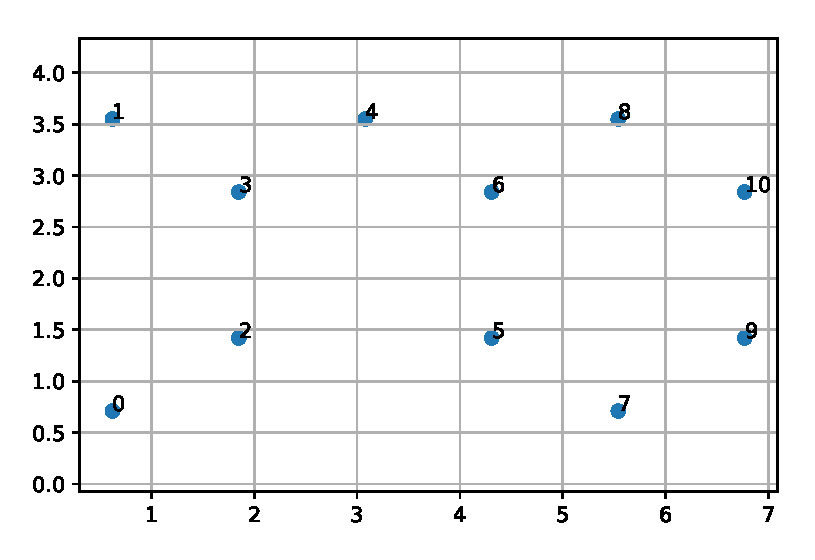
\includegraphics[width=\textwidth]{Figures/basicstructure.eps}
		\caption{The basic structure plotted with indices\vspace{\baselineskip}}
		\label{basicstructure}
	\end{subfigure}\vspace{2mm}
	~ %add desired spacing between images, e. g. ~, \quad, \qquad, \hfill etc.
	%(or a blank line to force the subfigure onto a new line)
	\begin{subfigure}[b]{0.4\textwidth}
		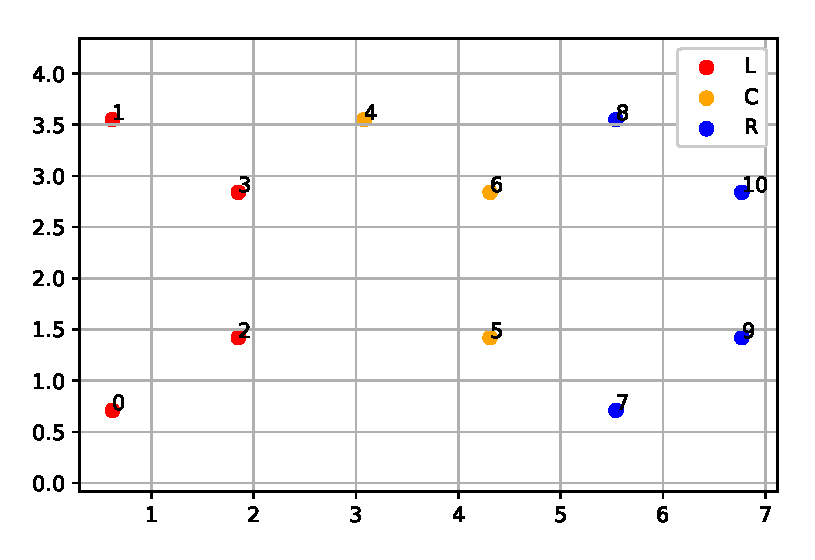
\includegraphics[width=\textwidth]{Figures/basicstructurewithcontacts.eps}
		\caption{The same structure now shown with indices marked red and blue as per users choice of contact atoms}
		\label{basicstructurewithcontacts}
	\end{subfigure}
	\caption{Figure showing the interface integrated into the script.}\label{interface}
\end{figure}
This allows the user to get the dimensions needed to define the left and right Hamiltonians so they can be picked out of the device Hamiltonian. From the left and right Hamiltonian the corresponding hopping matrices are defined using the \textit{Hop} function. Then the \textit{EnergyRecursion} is used to obtain the Green's function for the device. This function is a more elaborate version of the earlier mentioned \textit{RecursionRoutine}. It uses the old recursion routine to calculate the self energies for the left and right cells (\(\mathbf{\Sigma}_{L/R}\)) (see line 164-165 \cref{engrec}) and then uses those to calculate the device Green's function \(\textbf{G}_D\) as well as the left and right rate matrices \(\mathbf{\Gamma}_{L/R}\), using the equations \cref{rateeq}, \cref{devicegreens} (see \cref{engrec} line 176-179).\im{Listings/Functions.py}{156}{185}
\vspace{-1\baselineskip}
\captionof{listing}{lalala\label{engrec}}\vspace{\baselineskip}The output of the energy recursion function is the two rate matrices (left and right) as well as the device Green's function and as per \cref{transeq} the matrices needed for transmission have been obtained. As seen in \cref{transfunc} the transmission function \textit{Transmission} simply carries out the matrix product and subsequent trace of the resulting matrix and outputs a range of transmission probabilities which is then plotted against an energy range. Do mind that this is still just 1D in the sense that the transmission only moves in one direction. A plot of the transmission for such a simple 1D system (the one in \cref{basicstructure}) can be seen in \cref{alphatrans}.\im{Listings/Functions.py}{188}{195}
\vspace{-1\baselineskip}
\captionof{listing}{lalala\label{transfunc}}\vspace{\baselineskip}
\begin{figure}[ht]
    \centering
    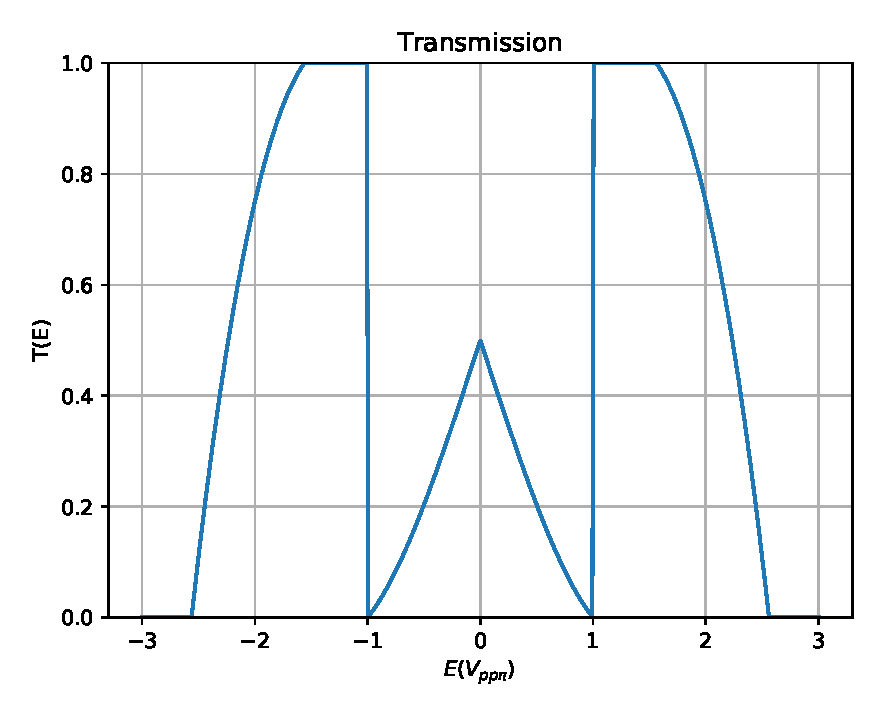
\includegraphics[width =0.5\textwidth]{Figures/alphaTE.eps}
    \caption{Transmission plot for the system in \cref{interface}}
    \label{alphatrans}
\end{figure}
\subsubsection{Development of transmission to 2D}
Lastly the transmission routine needs to be generalised so it can handle transport in two directions. The most convenient approach is to work with five real space unit cells as a starting point. One center cell, a right and a left cell representing the contacts and then two additional cells on the left and right, representing the rest of the contact region. This would be the minimum amount of cells needed to generalise the transmission. One might have more center cells if the structure changes from one of those cells to the other. First these five unit cells will be defined using already developed tools. Then a big Hamiltonian, including all coordinates from the five cells representing real space are created, again using existing functions. One could call this big Hamiltonian \(\textbf{H}_{\text{Bigreal}}(xyz_0,xyz_0)\). It is a function of two sets of identical coordinates, namely the ones used to create the Hamiltonian itself. This has also been the case for all previous calculations, but the following steps will make it clear why it is explicitly stated for this Hamiltonian. The left/right on-site Hamiltonians and hopping matrices can thus be picked out of \(\textbf{H}_{\text{Bigreal}}(xyz_0,xyz_0)\) as before to get the Green's functions, self energies for transmission in real space, just as in the previous section. But instead, before the Green's function, self energies and transmission is calculated, the left/right onsite-Hamiltonian as well as their hopping matrices are defined as functions of a variable \(k\) and the hopping will additionally have a phase added which depends on a variable \(q\). As an example the following is the equation for the full right side Hamiltonian using the right on-side Hamiltonian with its hopping matrices: \(\textbf{H}_R(k,q) = \textbf{V}_R(k)e^{iq}+\textbf{V}^{\dagger}_R(k)e^{-iq}+\textbf{h}_R(k)\). The \(k\) represents .... and the \(q\) represents ..... The next part is to obtain
the hop from \(\textbf{H}_{\text{Bigreal}}(xyz_0,xyz_0)\) to an equal cell in the other (transverse) direction, so that the transmission will become truly 2D. Firstly the hopping between \(\textbf{H}_{\text{Bigreal}}(xyz_0,xyz_0)\) and a transversely shifted Hamiltonian is defined as \(\textbf{W} = \textbf{H}_{\text{Bigtrans}}(xyz_0,xyz_1)\) (Here using \textbf{W} as not to confuse it with \textbf{V} which is hopping between cells in real space). Note that the index of one of the coordinate sets have changed to 1. This corresponds to a shift by the lattice vector going in the transverse direction to that of the transmission direction defined in 1D. With the hopping matrices for the transverse direction defined a Hamiltonian dependent on \(k\)-point values can be defined as:\begin{align}
    \textbf{H}(k) &= \textbf{h}+\textbf{W}e^{ik}+\textbf{W}^{\dagger}e^{-ik}\\
    &= \textbf{H}_{\text{Bigreal}}(xyz_0,xyz_0) + \textbf{H}_{\text{Bigtrans}}(xyz_0,xyz_1)e^{ik}+\textbf{H}_{\text{Bigtrans}}^{\dagger}(xyz_0,xyz_1)e^{-ik}
\end{align}
Now a Hamiltonian, dependent of a variable \(k\) has been defined, and thus it is now possible to get self energies, Green's functions that is \(k\)-dependent as well as a transmission (also \(k\)-dependent) which can be found for different \(k\)-points i.e. different points in the transverse direction (inverse space). This hereby concludes the all the initial effort to develop a code which can do calculations of different points of interest (Green's function plots, band structures and transmission) in a two dimensional material such as NPG. Following is a walk through as to how this last step has been implemented through code programming. 

\section{Exploring functionality of GNR bridges}\label{testsec}
%!TEX root = ../Main.tex
In this section a range of tests will be conducted on different NPG structures in order to uncover the effect of chemical modification of the bridges between the Graphene Nano Ribbons (GNRs) in the NPG. From an applied perspective, one of the main motivations is to find out how these bridges can be chemically modified in order to control the current through the material. A recent study\cite{unpub}, submitted for publication in JACS\footnote{\href{https://pubs.acs.org/journal/jacsat}{Journal of American Chemical Society}}, has shown how one could possibly confine current flow to a single GNR channel by modification of bridges between GNR's in NPG utilising \textit{Quantum Interference} (QI) effects (See \cref{studyfig3} b)). This provides a solution to an important requirement in carbon-based nano circuitry design, namely nano confinement of electron flow. The study was focused on the difference in effect of having \textit{meta} and \textit{para} bridges between GNR's. Meta and para bridges are essentially benzene rings connected in two different ways (See \cref{Metaparastructfig}). The meta and para bridges are 'static' cases in the sense that once made through organic synthesis, they are not interchangeable. However, if the bridges are functionalised with oxygen\cite{Soler_2002} they become sensitive to f.ex. hydrogenation in basic/acidic environments, which tends to affect QI. Thus by hydrogenation it should be possible to tune the electrical properties of the material and make it sensitive to external environments. Studies\cite{li_single_2019} show that hydrogenation of specific sites on nanometer scale is possible experimentally. By the use of the functions developed in previous sections, this section will try to uncover what happens when oxygen is bonded to the benzene rings in the meta and para bridges. Subsequently hydrogenation of the oxygen will be tested. Following is a section introducing para and meta NPG in detail.
\begin{figure}[h]
    \renewcommand\thesubfigure{\arabic{subfigure}}
	\centering
	\begin{subfigure}[b]{0.9\textwidth}
	    \centering
	    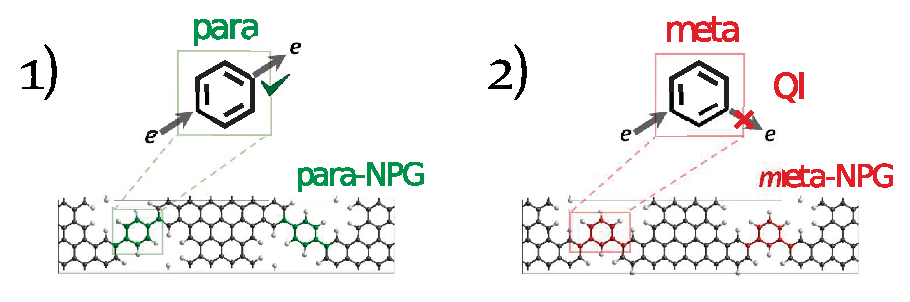
\includegraphics[width=0.8\textwidth]{Figures/Metaparagraphic.eps}
	    \caption{}
    	\label{Metaparastructfig}
    \end{subfigure}
    \vskip
    \begin{subfigure}[b]{0.9\textwidth}
        \centering
	    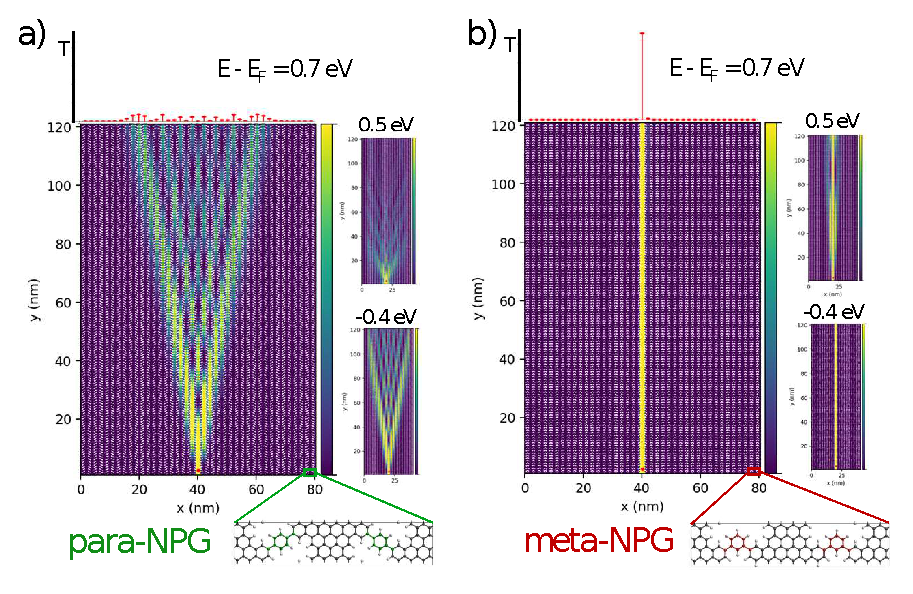
\includegraphics[width = 0.7\textwidth]{Figures/Fig_3.eps}
	    \caption{}
	    \label{studyfig3}
	\end{subfigure}
\caption{1: a) showing the para NPG, b) showing the meta NPG. 2: Figure showing the currents through the GNR's in a large peace of NPG. Note how the current is spread across GNR's with the para bridge a) and confined to a single GNR with meta bridge b). Used with permission from Isaac Alcón Rovira.}
\label{studyfigs}
\end{figure}
\subsection{Bridge effects in para-NPG and meta-NPG}\label{metaparasection}
In broad terms the difference in the \textit{meta} and \textit{para} structures lies in the path an electron will travel through the benzene ring to get across the bridge between GNR's in NPG. In the para bridge, the path across the aromatic ring is symmetric and so the electron will pass above or below with equal phase. Since the para bridge has three bonds in each direction across the ring, the path length in the para bridge is the same on each side (See \cref{Metaparastructfig} a)). This will cause constructive quantum interference of the states once the waves meet on the other side of the ring. For para NPG this causes electronic coupling between the GNR channels. In the meta bridge, the way across the aromatic ring is not symmetric in the sense that there is two bonds across the path below and four bonds across on the path above (See \cref{Metaparastructfig} b)). This will cause a shift by half a wavelength between the two paths and thus create destructive quantum interference between waves meeting on the other side of the ring. This causes electronic decoupling between GNR channels, allowing for confinement of injected currents in a single GNR channel\cite{unpub} (see \cref{studyfig3}). In \cref{metapara} band plots as well as transmission plots from the study\cite{unpub} are shown for para and meta NPG. In the band plots the two sets of valence/conduction bands around the Fermi level shows band splitting for para and interference for meta NPG. Looking at the transmission plots next to the band plots one can see there is transmission and thus coupling of the states between the GNR's for para. The area between the two peaks at \SI{0.5}{\electronvolt} and  \SI{1.2}{\electronvolt} show transport between the GNR's. In the transmission plot for meta the transmission is supressed (\cref{metapara} right). The transmission plot the area between the two peaks is now pretty much 0. This means GNR's are electrically decoupled in meta system. To summarise these results qualitatively: Splitting of the bands in the band plots, corresponds to effective coupling of the GNR's. Bands on top of each other, showing QI, corresponds to decoupling of the GNR's and thus electric confinement of injected currents on NPG in single GNR channels (see \cref{studyfig3}). In the following sections, band plots will mainly be used to show results. Therefore one should keep in mind how the band structures, qualitatively, relate to transmission. In \cref{appfigs}, \cref{allbands} a figure obtained from the developed functions with band plots of normal, para and meta NPG can be seen.
\begin{figure}[ht]
	\centering
	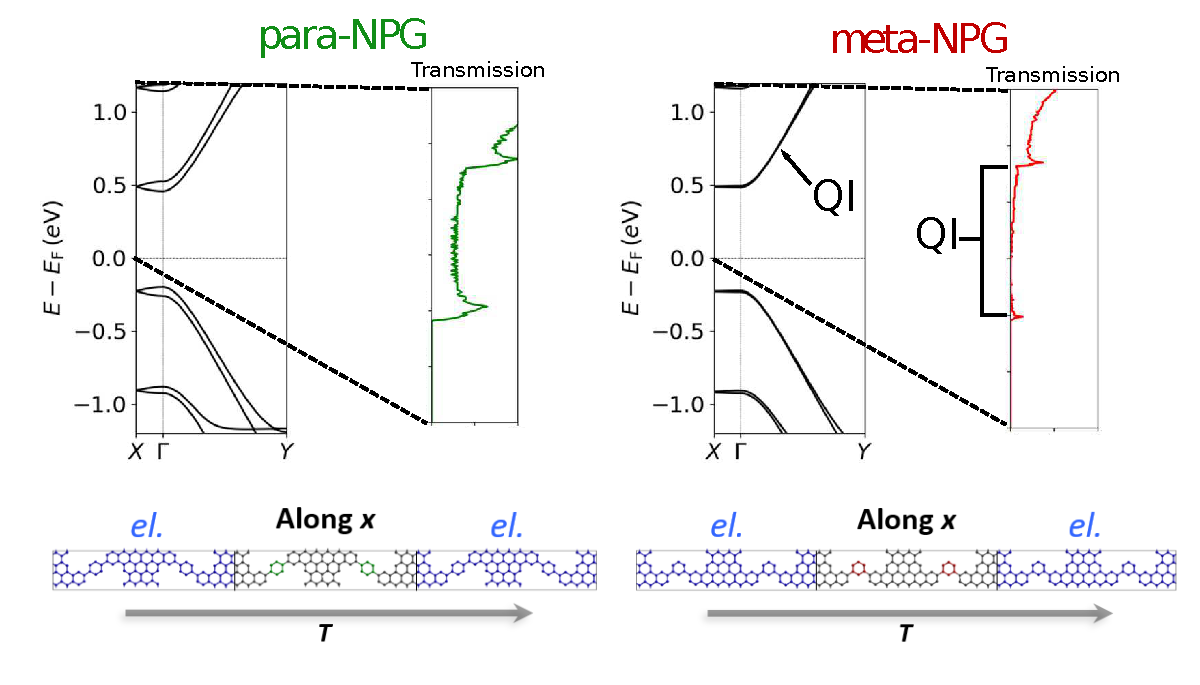
\includegraphics[width=0.8\textwidth]{Figures/metapararesultdraft.eps}
	\caption{Figure showing band plots and transmission plots for para and meta NPG. In the bottom of each plot is a schematic showing which way the transmission occurs in relation to the NPG. Used with permission from Isaac Alcón Rovira}
	\label{metapara}
\end{figure}
\newpage
\subsection{Tests with oxygen modified meta and para-NPGs}\label{test1}
The tests consist of two kinds of chemical modification. Firstly it will be bonding oxygen sites to the meta and para NPG (Addition of Oxygen will be simulated by addition of another carbon site to the structure, effectively adding another pi-electron). Secondly simulations of hydrogenation will be done by bonding hydroxide groups to the bridges. These modifications will be carried out separately. Because of the complex nature of DFT the band plots obtained via DFT makes it hard to interpret what is actually going on in the system chemically. Therefore the aim is to show that using the methods developed, based on tight-binding models, it is possible to reproduce bands structures calculated from DFT. If successful, it will provide a much easier way to understand the effect of the implemented chemical modification compared to the DFT approach. Band plots, as well as some on-site potential maps, calculated with DFT has been provided by supervisor Isaac Alcón Rovira for comparison. The geometries, used for calculations, are provided by supervisor Isaac Alcón Rovira and have been optimised by DFT using the SIESTA package\cite{Soler_2002} and the PBE functional\cite{perdew1996a}.
\subsection{Test 1: Para-O\mathinhead{_4}{_4}-NPG}
The first test is considering the Para-O\(_4\)-NPG. The basic structure is para-NPG where 4 oxygen sites are bonded, two on each benzene ring (See \cref{PS4OOW} ). Starting by looking at the resulting DFT plot in \cref{PS4ODFT} the first thing to notice is that the valence bands show QI and thus decouples the GNR's. So in spite having a para bridge, which normally gives coupling, decoupling occurs when oxygen is bonded to the bridges. Our first assumption to simulate the effect of such oxygen functionalisation is to add those atoms as active \(p_z\)-orbitals in our pi-conjugated system, using the standard parameters (i.e. as for carbon atoms - specifically the on-site potential and hopping value). As a baseline the potential of these atoms are thus the same. Moreover, the hydrogen, included in the provided optimised geometries, will be removed before any calculations take place. In \cref{PS4Odevnomod} one can see the resulting band structure plot, using such and electronic model and the DFT optimized structure. The band plot does not show much resemblance with the one obtained, using DFT. It is pretty much symmetric around the Fermi level and it is hard to make out whether there is coupling or decoupling between GNR's, based on the reasoning discussed in \cref{metaparasection}. Taking a look at the DFT-calculated potential map of \cref{potmapPS4O}, the sites where the oxygen is bonded, have a potential much different from that of the rest of the system (the four dark blue spots). As mentioned, the baseline of the method does not take into account differentiating on-site potentials within a cell. So to compensate for this, the on-site potential of the four bonded oxygen is changed. In \cref{PS4Odevmod} one can see the resulting band plot after the on-site potential of the bonded oxygen has been changed to \SI{-0.50}{\electronvolt}. The resulting band plot resembles the DFT calculations much more. There is now QI in the valence bands which means decoupling of the GNR's. To summarise the results the tests showed significant qualitative agreement with the DFT calculation. This helps to uncover the main effect of functionalisation of para-NPG with oxygen. Knowing that the added \(p_z\) electrons where participating in the pi-conjugated system, those orbitals had to be accounted for in the developed model by addition of extra sites. However, to qualitatively reproduce the DFT results, the on-site potential of those extra sites had to be lowered by \SI{-0.5}{\electronvolt}. This helped to explain why functionalisation with oxygen only affects the valence band of NPG and not the conduction band. In addition the developed method also reproduced the flat bands seen around the Fermi level in the DFT calculation (The developed method showed bands exactly at the Fermi level). In broad terms, these bands are related to benzene bridge in the NPG, but they originate because of the presence of the bonded oxygen. The oxygen do have an dispersive effect on the valence electrons of NPG, but they also seem to be localised in nature, which is why the flat bands occur.   
\begin{figure}[H]
	\centering
	\begin{subfigure}[b]{0.8\textwidth}
		\centering
		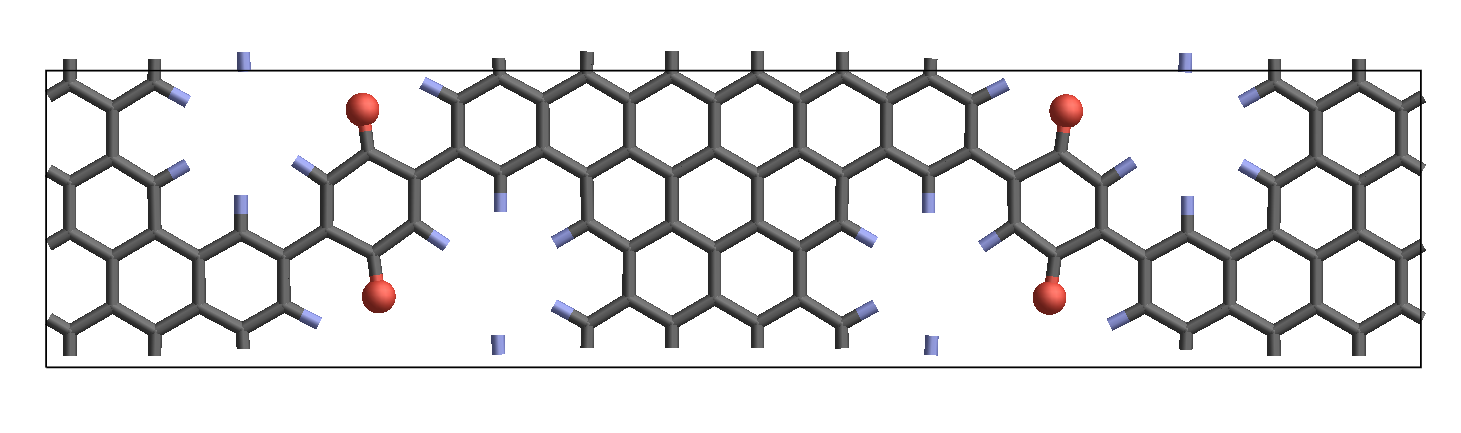
\includegraphics[width=0.8\textwidth]{Figures/para_O4.png}
		\vspace{-1\baselineskip}
		\caption{}
		\label{PS4OOW}
	\end{subfigure}
	\vskip
	\begin{subfigure}[b]{0.3\textwidth}
		\centering
		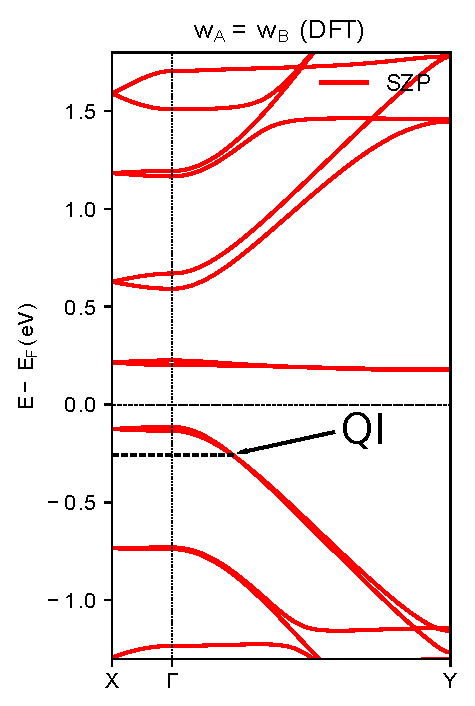
\includegraphics[width=0.8\textwidth]{Figures/PS4ODFT.eps}
		\vspace{-1\baselineskip}
		\caption{}
		\label{PS4ODFT}
	\end{subfigure}
	\hspace{-20pt}
	\begin{subfigure}[b]{0.3\textwidth}
		\centering
		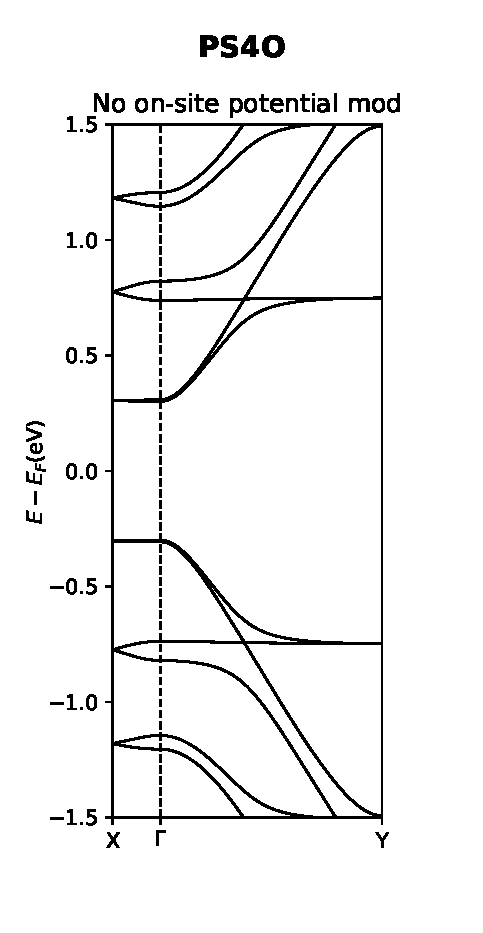
\includegraphics[width=0.8\textwidth]{Figures/PS4Onomod.eps}
		\vspace{-2\baselineskip}
		\caption{}
		\label{PS4Odevnomod}
	\end{subfigure}
	\hspace{-30pt}
	\begin{subfigure}[b]{0.3\textwidth}
		\centering
		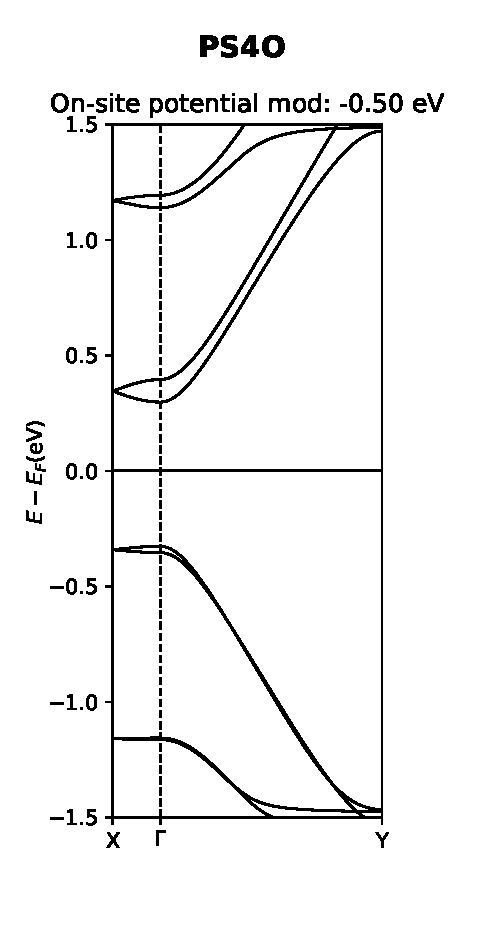
\includegraphics[width=0.8\textwidth]{Figures/PS4Omod.eps}
		\vspace{-2\baselineskip}
		\caption{}
		\label{PS4Odevmod}
	\end{subfigure}
	\vskip
	\begin{subfigure}[b]{0.8\textwidth}
	    \hspace{50pt}
		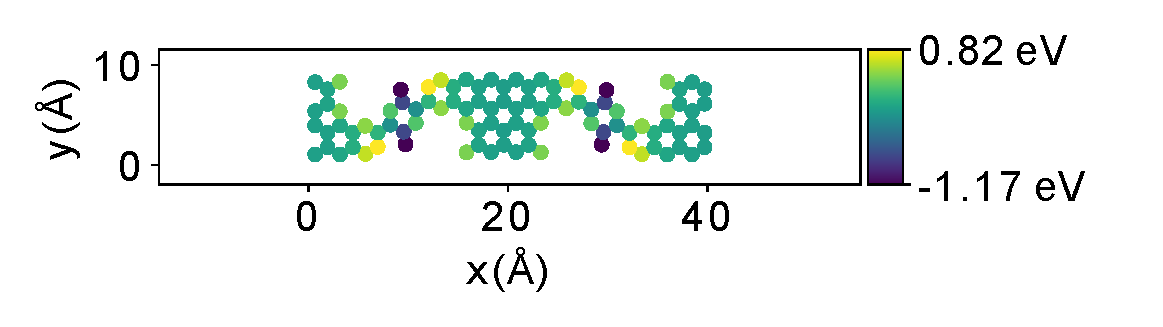
\includegraphics[width=0.8\textwidth]{Figures/PS4O.eps}
		\vspace{-0.5\baselineskip}
		\caption{}
		\label{potmapPS4O}
	\end{subfigure}
	\caption{a) Overview of the system with carbon (grey), oxygen (red) and hydrogen atoms (blue) and highlighting the added oxygen or hydroxide groups as spheres. b) Band structure obtained using DFT. c) Band structures obtained using developed program with no on-site potential mods. c) Band structures obtained using developed method with the on-site potential changed to \SI{-0.5}{\electronvolt}. d). Potential map of the system.}
	\label{PS4O}
\end{figure}
\subsection{Test 2: Para-(OH)\mathinhead{_4}{_4}-NPG}\label{test2}
Next test will be with the Para-(OH)\(_4\)-NPG system. Again the basic structure is para-NPG with bonded oxygen, but here the aim is to simulate hydrogenation, so therefore the oxygen atoms added will become hydroxide groups (See \cref{PS4OHOW}). The DFT plot in \cref{PS4OHDFT} shows a band splitting in the valence/conduction bands, so the GNR's have been coupled again. Here the first approach is to use the succesfull method reproducing the DFT results in \cref{test1}: i.e. considering oxygen positions as active \(p_z\) ortry to use the applied on-site potential for the bonded oxygen from the previous test (\cref{test1}) as a baseline. This is on the assumption that oxygen still contribute to the pi-conjugated system. In \cref{PS4OHmod2} the resulting band plot can be seen. It shows exactly the same as \cref{PS4Odevmod}. What one can conclude for this is that even though the geometries provided are optimised with DFT specifically for each system, the developed method does not distinguish the small differences in distance between atoms, which leads to hopping. The result is that, seen from a tight-binding point of view, the geometries are the same initially even though they have been optimised individually with DFT. Therefore the resulting plots are identical. A natural way to compensate for this is to change the on-site potential by a value significantly lower, so that hopping can occur. Using the potential plot in \cref{potmapPS4OH} as a guide the on-sties of the oxygen are changed to \SI{-2}{\electronvolt}. The resulting plot can be seen in \cref{PS4OHdevmod}. The plot show good agreement with the DFT. The bands have shifted again and the GNR's are coupled. This means hydrogenation decouples the oxygen, so by lowering the on-site potential of one can get effective decoupling of oxygen. As seen this gives a satisfying result. Now that it is known that hydrogenation decouples the oxygen, a last hypothesis is that by removing the hydroxide group entirely, before calculation, the result will be similar to \cref{PS4OHdevmod}. In \cref{PS4OHremove} the resulting plot can be seen. As hypothesised, the resulting band plot show resemblance with both the DFT and \cref{PS4OHdevmod}. So the decoupling of oxygen by hydrogenation can be simulated simply by removing the hydroxide group entirely. Again there is shifts in the bands and thus coupling of the GNR's. This means that the developed method can uncover what happens chemically when the NPG is hydrogenated and it can do so in a simple manner.
\begin{figure}[H]
	\centering
	\begin{subfigure}[b]{0.8\textwidth}
		\centering
		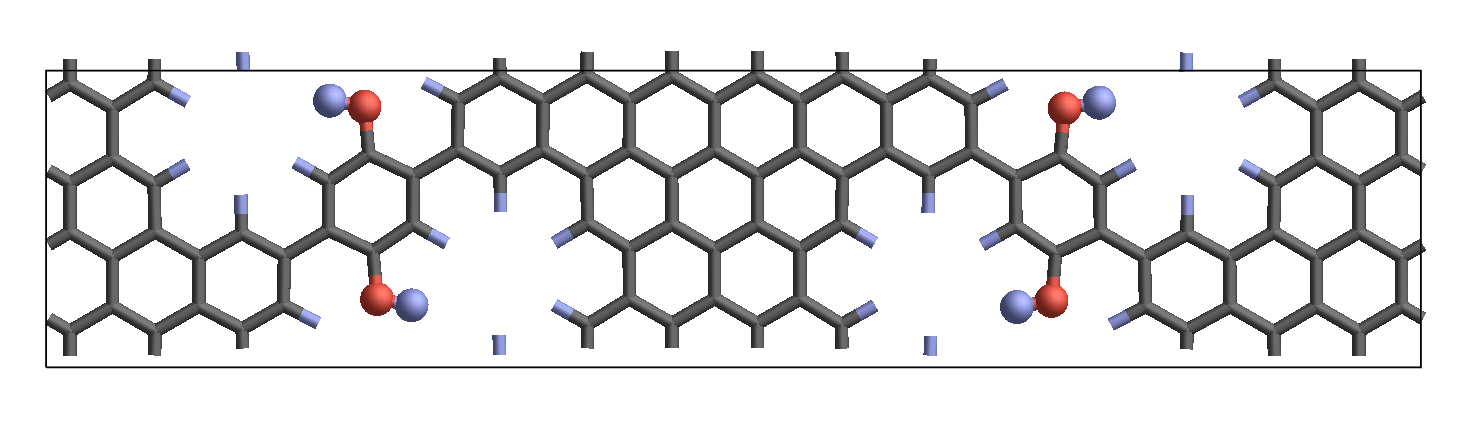
\includegraphics[width=0.8\textwidth]{Figures/para_OH4.png}
		\vspace{-1\baselineskip}
		\caption{}
		\label{PS4OHOW}
	\end{subfigure}
	\vskip
	\begin{subfigure}[b]{0.25\textwidth}
		\centering\hspace{-20pt}
		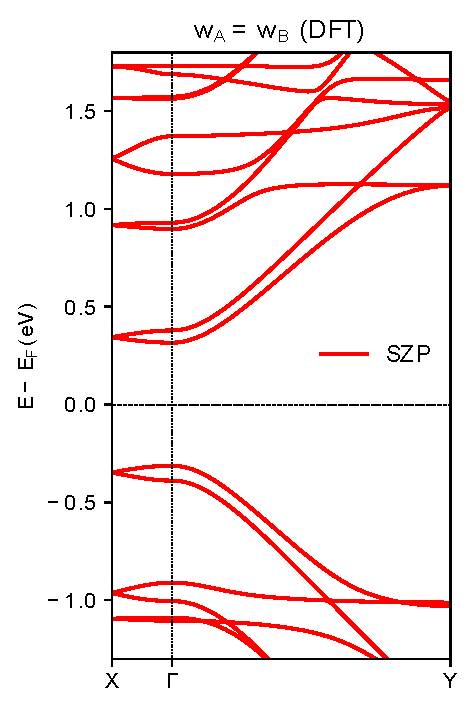
\includegraphics[width=0.8\textwidth]{Figures/PS4OHDFT.eps}
		\vspace{-1\baselineskip}
		\caption{}
		\label{PS4OHDFT}
	\end{subfigure}
	\hspace{-20pt}
	\begin{subfigure}[b]{0.25\textwidth}
		\centering
		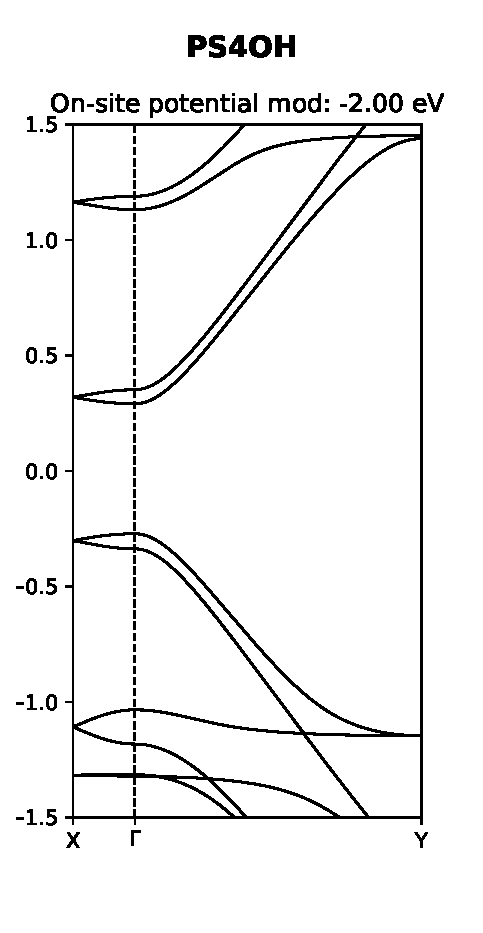
\includegraphics[width=0.8\textwidth]{Figures/PS4OHmod2.eps}
		\vspace{-2\baselineskip}
		\caption{}
		\label{PS4OHmod2}
	\end{subfigure}
	\hspace{-20pt}
	\begin{subfigure}[b]{0.25\textwidth}
		\centering
		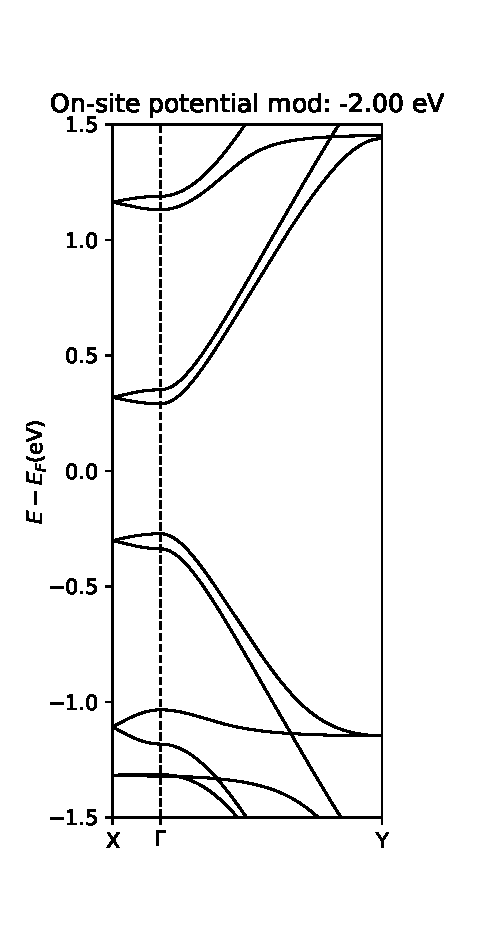
\includegraphics[width=0.8\textwidth]{Figures/PS4OHmod.eps}
		\vspace{-2\baselineskip}
		\caption{}
		\label{PS4OHdevmod}
	\end{subfigure}
	\hspace{-20pt}
	\begin{subfigure}[b]{0.25\textwidth}
		\centering
		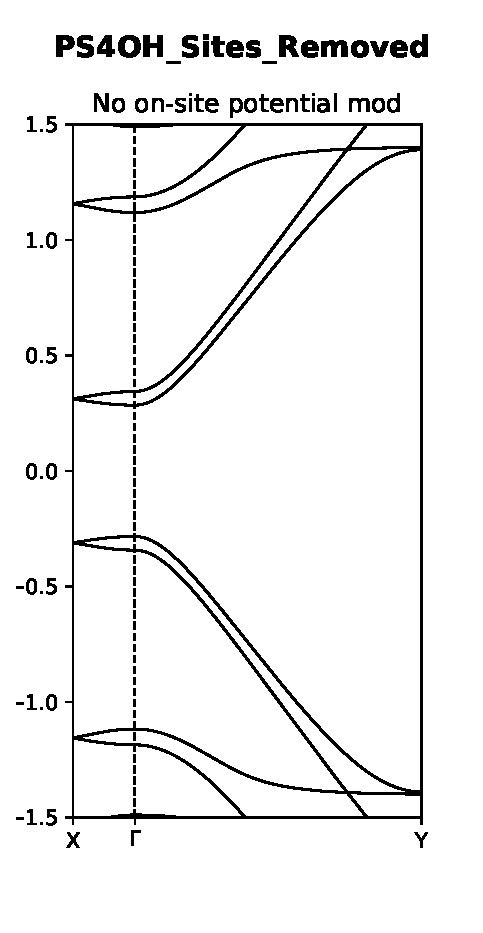
\includegraphics[width=0.8\textwidth]{Figures/PS4OHSitesRemoved.eps}
		\vspace{-2\baselineskip}
		\caption{}
		\label{PS4OHremove}
	\end{subfigure}
	\vskip
	\begin{subfigure}[b]{0.8\textwidth}
		\centering\hspace{30pt}
		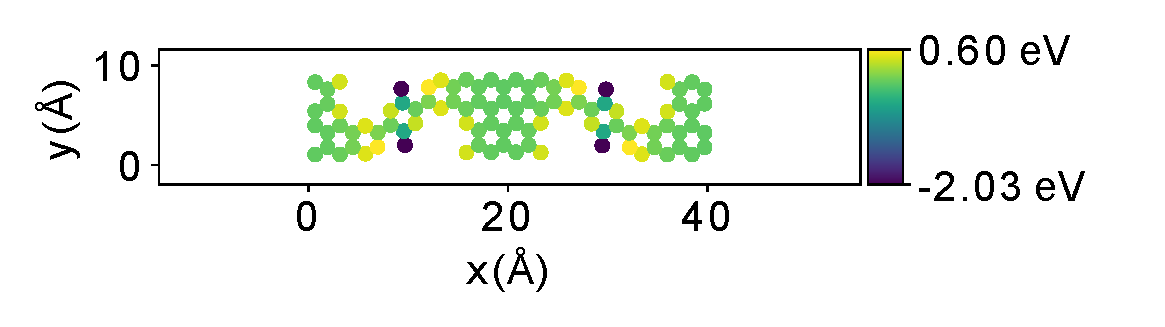
\includegraphics[width=0.8\textwidth]{Figures/PS4OH.eps}
		\vspace{-0.5\baselineskip}
		\caption{}
		\label{potmapPS4OH}
	\end{subfigure}
	\caption{a) Overview of the system with carbon (grey), oxygen (red) and hydrogen atoms (blue) and highlighting the added oxygen or hydroxide groups as spheres. b) Band structure obtained using DFT. c) Band structures obtained using developed program with with on-site potential changed to \SI{-0.5}{\electronvolt}. d) Band structures obtained using developed method with on-site potential changed to \SI{-2}{\electronvolt}. e) Band structures obtained using the developed method with sites removed. f) Potential map of the system.}
	\label{PS4OH}
\end{figure}
\subsection{Test 3: Meta-NPG with oxygen added symmetrically}\label{test3}
Moving on to the meta NPG, the test is going to be exactly the same as \cref{test1}. To see the structure of the system look in \cref{MS2OOW}. Recall from \cref{metaparasection} that the meta NPG gives rise to QI and thus decoupling of the GNR's. However as seen in \cref{test1}, functionalising the bridges with oxygen caused some quantum interference in the para and thus decoupling of the GNR's in para NPG. The expected outcome of this test is that by functionalising the meta NPG bridges with oxygen will give rise to shifts in the bands and coupling of the GNR's. First the DFT plot in \cref{MS2ODFT} show that there is indeed a shift in the valence and that it is bigger than the shift in the conduction band. So by functionalising with oxygen the effect is most prevalent at the valence band for both para and meta. In \cref{MS2Odevnomod} the blot for the system with no modification is shown. Here one can also so see shifts in the valence and conduction bands. However, the plot is totally symmetric around 0 so it is not entirely accurate. Again the potential map in \cref{potmapM2SO} is used to get the on-site potential of the oxygen, so that they can be modified with the developed method. The result is seen \cref{MS2Odevmod}. Now the band plot shows a shift of the bands downwards, just like the DFT and the valence bands have a bigger shift compared to the conduction bands. So effectively the GNR's are coupled.
\begin{figure}[H]
	\centering
	\begin{subfigure}[b]{0.8\textwidth}
	    \centering
		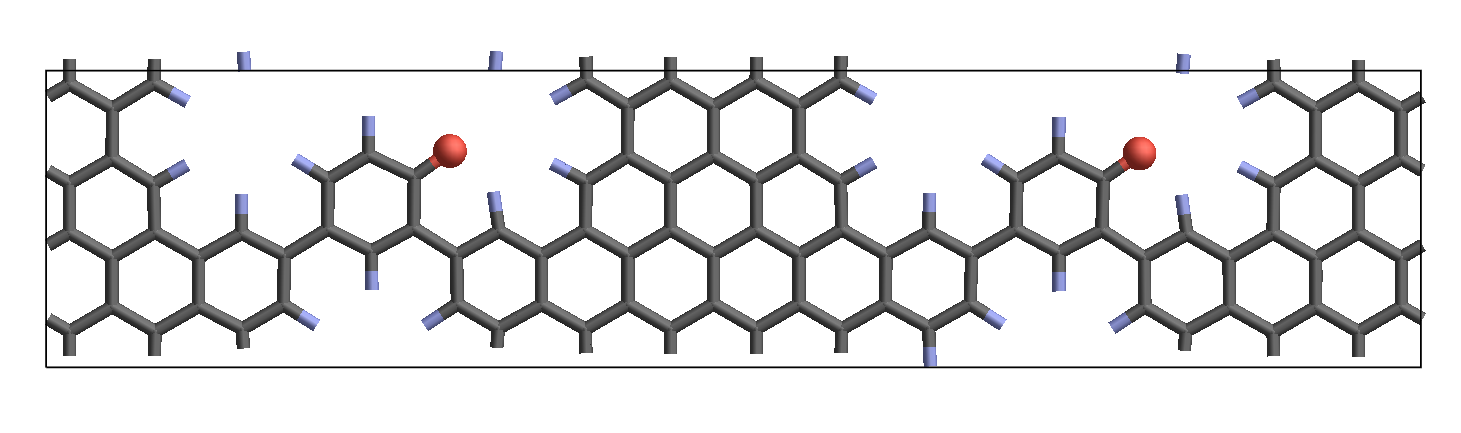
\includegraphics[width=0.8\textwidth]{Figures/meta_O4.png}
		\vspace{-1\baselineskip}
		\caption{}
		\label{MS2OOW}
	\end{subfigure}
	\vskip
	\begin{subfigure}[b]{0.3\textwidth}
		\centering
		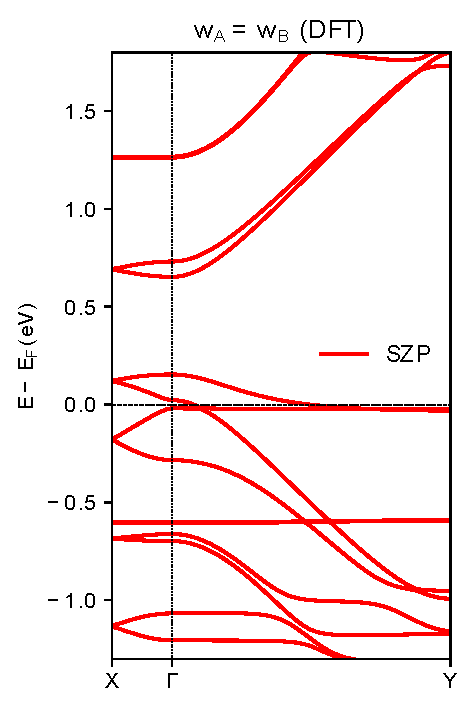
\includegraphics[width=0.8\textwidth]{Figures/MS2ODFT.eps}
		\vspace{-1\baselineskip}
		\caption{}
		\label{MS2ODFT}
	\end{subfigure}
	\hspace{-20pt}
	\begin{subfigure}[b]{0.3\textwidth}
		\centering
		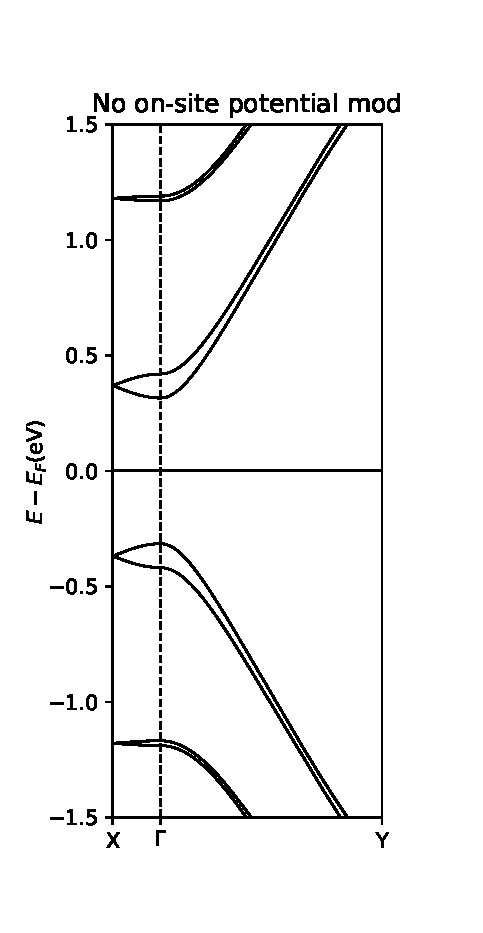
\includegraphics[width=0.8\textwidth]{Figures/MS2Onomod.eps}
		\vspace{-2\baselineskip}
		\caption{}
		\label{MS2Odevnomod}
	\end{subfigure}
	\hspace{-30pt}
	\begin{subfigure}[b]{0.3\textwidth}
		\centering
		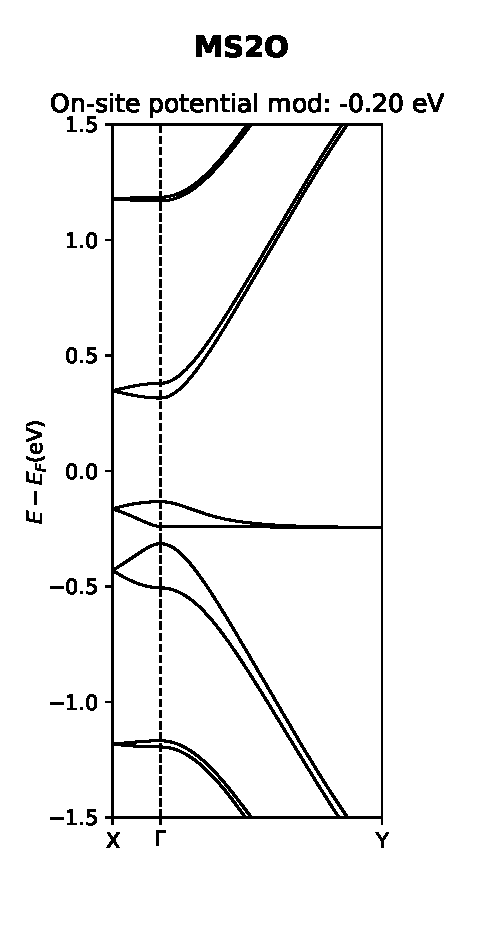
\includegraphics[width=0.8\textwidth]{Figures/MS2Omod.eps}
		\vspace{-2\baselineskip}
		\caption{}
		\label{MS2Odevmod}
	\end{subfigure}
	\vskip
	\begin{subfigure}[b]{0.8\textwidth}
	    \hspace{50pt}
		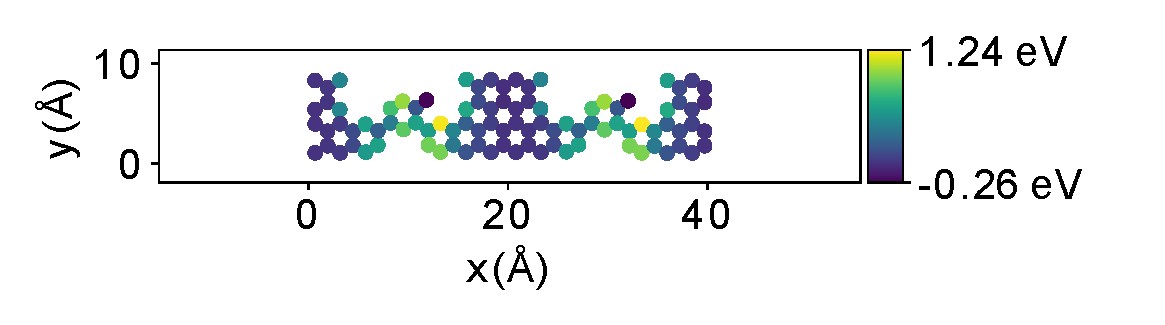
\includegraphics[width=0.8\textwidth]{Figures/MS2Opotmap.eps}
		\vspace{-0.5\baselineskip}
		\caption{}
		\label{potmapM2SO}
	\end{subfigure}
	\caption{a) Overview of the system with carbon (grey), oxygen (red) and hydrogen atoms (blue) and highlighting the added oxygen or hydroxide groups as spheres. b) Band structure obtained using DFT. c) Band structures obtained using developed program with no on-site potential mods. c) Band structures obtained using developed method with on-site potential changed to \SI{-0.2}{\electronvolt}. d) Potential map of the system.}
	\label{MS2O}
\end{figure}
\subsection{Test 4: Simulating hydrogenation of meta-NPG with symmetrically added oxygen}\label{test4}
The fourth and final test will be with the same approach as \cref{test2} only here the hydrogenation is of the meta-NPG with oxygen bonded symmetrically (See \cref{MS2OHOW}). Here one would expect to see QI and decoupling of the GNR's again as the system is hydrogenated, following the logic of the other tests. The DFT plot in \cref{MS2OHDFT} shows QI for both valence and conduction bands. Again the first plot produced, using the developed method, will be using the on-site modification from \cref{MS2Odevmod} as a baseline. The resulting plot can be seen in \cref{MS2OHdevmod2}. As expected it is identical to that of \cref{MS2Odevmod}. There is a bigger shift in the valence band and the GNR's are coupled. So the on-site potential is lowered with a value according to \cref{potmapMS2OH} and the result can be seen in \cref{MS2OHdevmod}. As expected the plot is in good agreement with DFT, showing effective decoupling of oxygen and thus decoupling of GNR's just like the unmodified meta NPG discussed in \cref{metaparasection}. Finally by removing the hydroxide group entirely, using the developed method afterwards, the resulting band plot in \cref{MS2OHremove} is obtained. The result is also in good agreement with DFT. This again proves that the developed method can uncover the chemical effects of functionalisation with oxygen and subsequent hydrogenation in a simple manner.
\begin{figure}[H]
	\centering
	\begin{subfigure}[b]{0.8\textwidth}
		\centering
		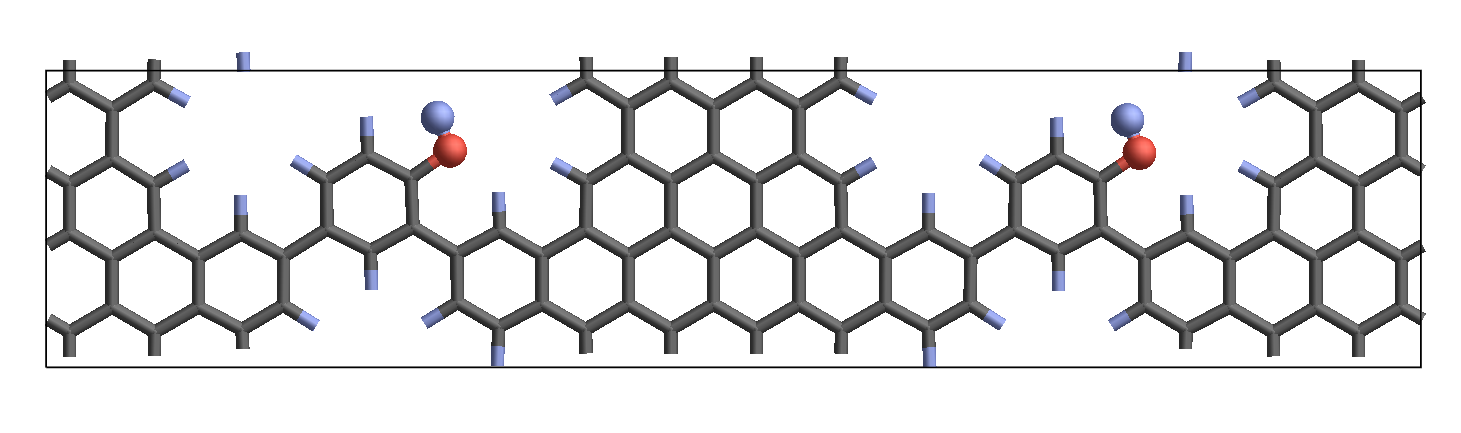
\includegraphics[width=0.8\textwidth]{Figures/meta_OH4.png}
		\vspace{-1\baselineskip}
		\caption{}
		\label{MS2OHOW}
	\end{subfigure}
	\vskip
	\begin{subfigure}[b]{0.25\textwidth}
		\centering
		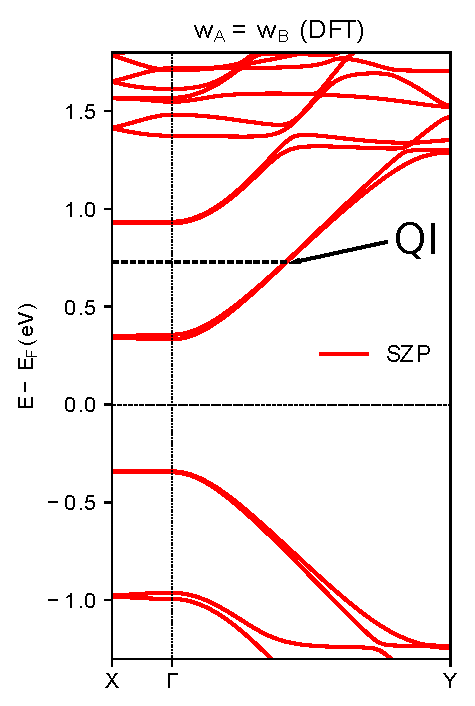
\includegraphics[width=0.8\textwidth]{Figures/MS2OHDFT.eps}
		\vspace{-1\baselineskip}
		\caption{}
		\label{MS2OHDFT}
	\end{subfigure}
	\hspace{-20pt}
	\begin{subfigure}[b]{0.25\textwidth}
		\centering
		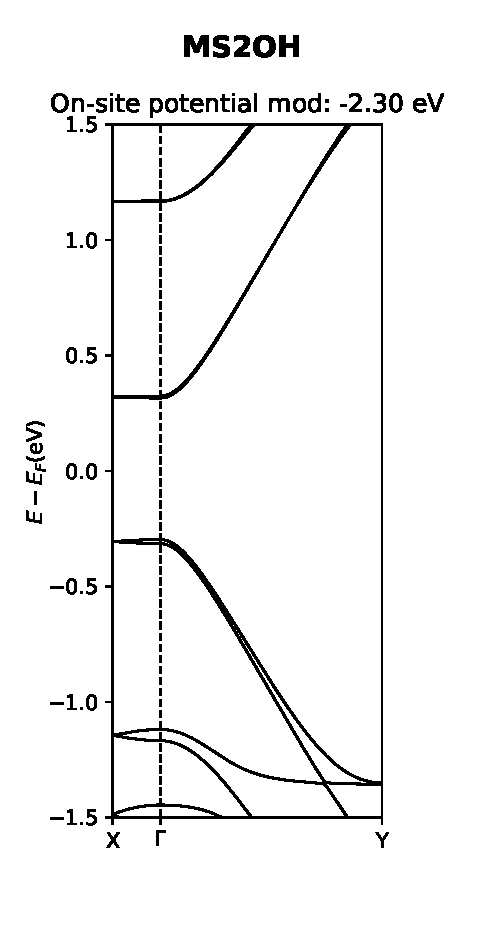
\includegraphics[width=0.8\textwidth]{Figures/MS2OHmod2.eps}
		\vspace{-2\baselineskip}
		\caption{}
		\label{MS2OHdevmod2}
	\end{subfigure}
	\hspace{-20pt}
	\begin{subfigure}[b]{0.25\textwidth}
		\centering
		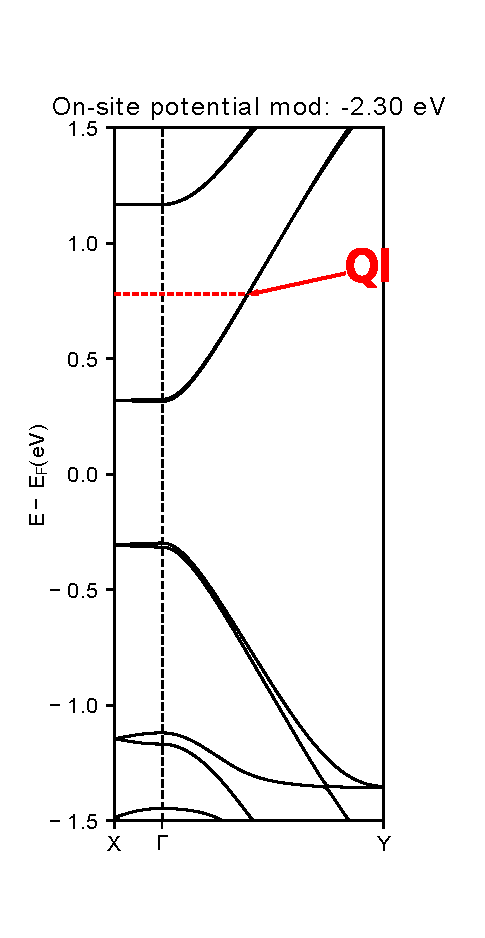
\includegraphics[width=0.8\textwidth]{Figures/MS2OHmod.eps}
		\vspace{-2\baselineskip}
		\caption{}
		\label{MS2OHdevmod}
	\end{subfigure}
	\hspace{-20pt}
	\begin{subfigure}[b]{0.25\textwidth}
		\centering
		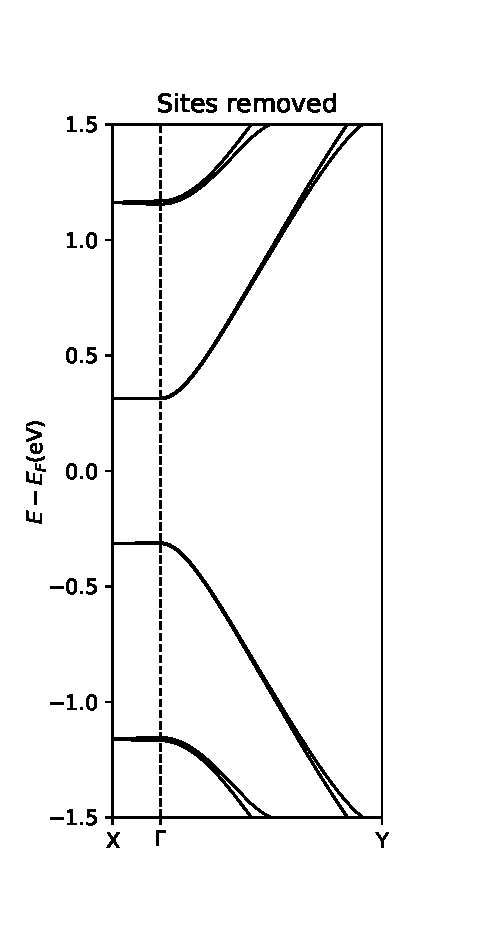
\includegraphics[width=0.8\textwidth]{Figures/MS2OHSitesRemoved.eps}
		\vspace{-2\baselineskip}
		\caption{}
		\label{MS2OHremove}
	\end{subfigure}
	\vskip
	\begin{subfigure}[b]{0.8\textwidth}
		\centering\hspace{30pt}
		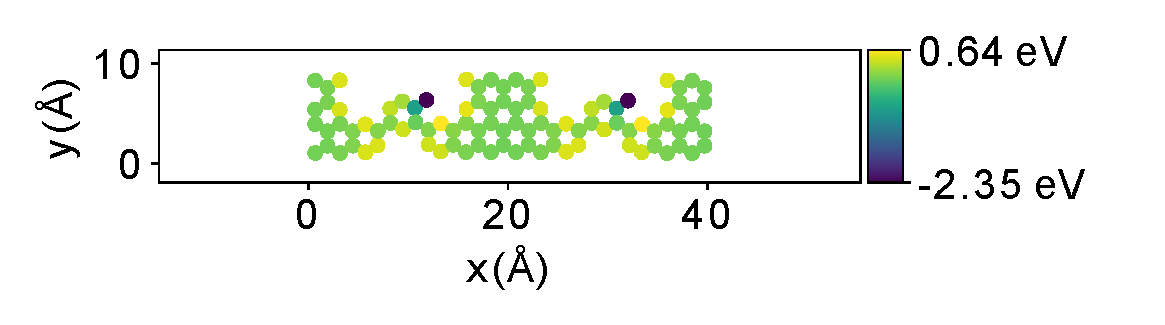
\includegraphics[width=0.8\textwidth]{Figures/MS2OH.eps}
		\vspace{-0.5\baselineskip}
		\caption{}
		\label{potmapMS2OH}
	\end{subfigure}
	\caption{a) Overview of the system with carbon (grey), oxygen (red) and hydrogen atoms (blue) and highlighting the added oxygen or hydroxide groups as spheres. b) Band structure obtained using DFT. c) Band structures obtained using developed program with with on-site potential changed to \SI{-0.2}{\electronvolt}. d) Band structures obtained using developed method with on-site potential changed to \SI{-2.3}{\electronvolt}. e) Band structures obtained using the developed method with sites removed. f) Potential map of the system.}
	\label{MS2OH}
\end{figure}
\subsection{Test summary}
For the para systems, the added oxygen introduced some QI to the system. It was possible to show that the developed program could reproduce the results obtained from DFT. This did require some adjustment to the on-site potential of the added oxygen. By hydrogenation of the oxygen it was shown that the system again returned to a shift in the bands. Again by adjusting the on-site potential it was possible to obtain results very close to the DFT calculation. The results are also comparable with the ones mentioned in \cref{metaparasection}. This shows that hydrogenation of oxygen can change the system to resemble regular para-NPG, even if it has oxygen bonded. The same can be said for the meta tests. All in all these results give a better, intuitive understanding of what happens with chemically with the systems and what effect it has on the electron transport in NPG. This is because all manipulations can be followed with ease and the results are easy to interpret. The tests have shown that it is possible to tune the electrical properties of chemically modified meta and para NPG by hydrogenation and thus providing a novel approach in designing sensitive nano circuitries, for f.ex. PH-sensors. This rounds off the summary of the test section. The section following will conclude the project as a whole.

\newpage
\begin{acknowledgments}
	The authors would like to thank...
\end{acknowledgments}
%End of text
% List of ToDos
%\listoftodos %Uncomment for list of todos
%Bibliography herunder:
%\newpage
\onecolumngrid
\bibliography{Bibliography}

\newpage
\listoffigures
\listoftables
\listoflistings
%\listoftodos
\newpage
 %Appendicer herunder:
% !TEX root = Main.tex
\appendix
\appendixpage
\addappheadtotoc
\section{Additional figures}\label{appfigs}
\begin{figure}[h]
	\centering
	\begin{subfigure}[b]{0.3\textwidth}
		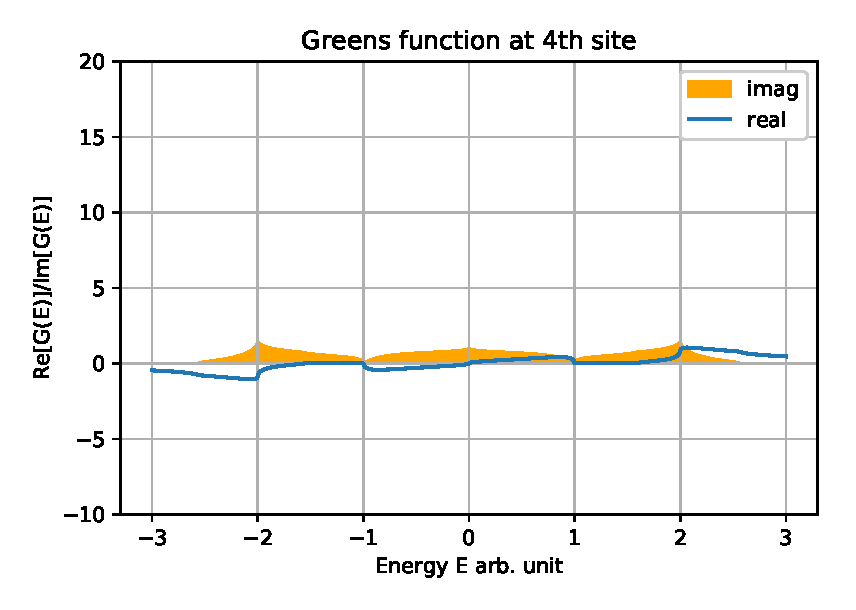
\includegraphics[width=\textwidth]{Figures/BetaimrealTE4.eps}
		\caption{Figure showing a plot of the Green's function at the 4th site}
		\label{4th}
	\end{subfigure}
	~ %add desired spacing between images, e. g. ~, \quad, \qquad, \hfill etc.
	%(or a blank line to force the subfigure onto a new line)
	\begin{subfigure}[b]{0.3\textwidth}
		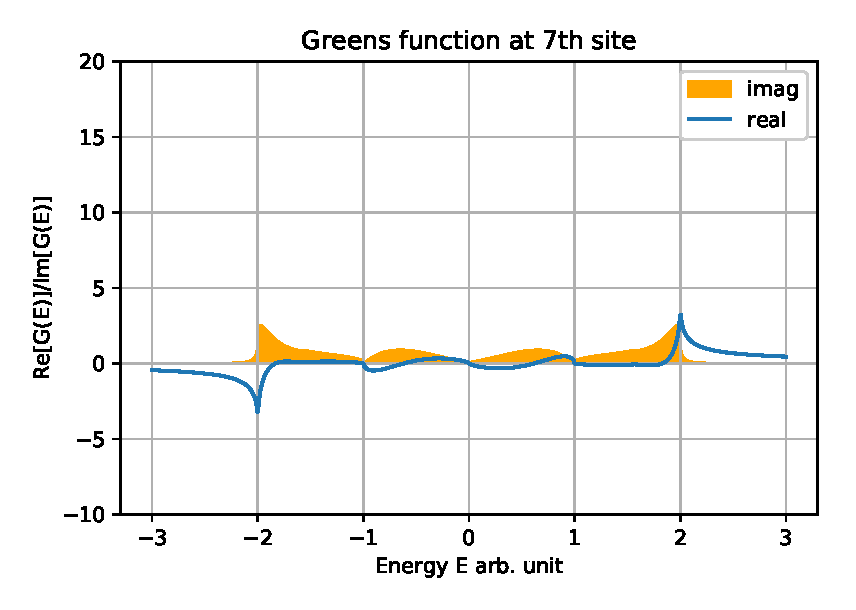
\includegraphics[width=\textwidth]{Figures/BetaimrealTE7.eps}
		\caption{Figure showing a plot of the Green's function at the 7th site}
		\label{7th}
	\end{subfigure}
	\caption{Two plots showing how the Green's function changes as the site is changed. The 4th and 7th sites are corresponding to atoms of those indices (4, 7) in \cref{pointplot}. Note how the LDOS changes (imaginary part) for the different sites.}\label{siteLDOSplot}
\end{figure}
\begin{figure}
	\centering
	\begin{subfigure}[b]{0.3\textwidth}
		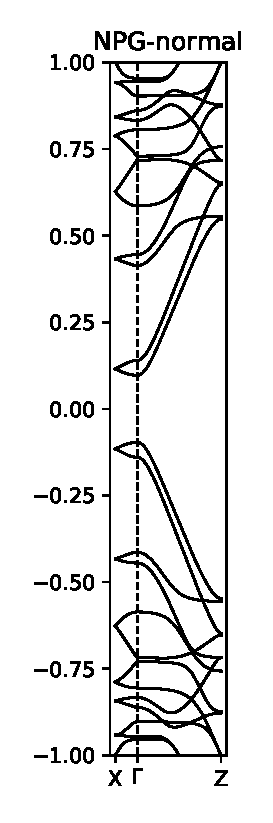
\includegraphics[width=\textwidth]{Figures/FabNPGBS.eps}
		\caption{Plot showing the band structure in the energy range \SI{-1.5}{\electronvolt} to \SI{1.5}{\electronvolt} for NPG with normal bridges between symmetry points \(X\) and \(Y\) with respect to \(\Gamma\)}
		\label{Fabbs}
	\end{subfigure}
	~ %add desired spacing between images, e. g. ~, \quad, \qquad, \hfill etc.
	%(or a blank line to force the subfigure onto a new line)
	\begin{subfigure}[b]{0.3\textwidth}
		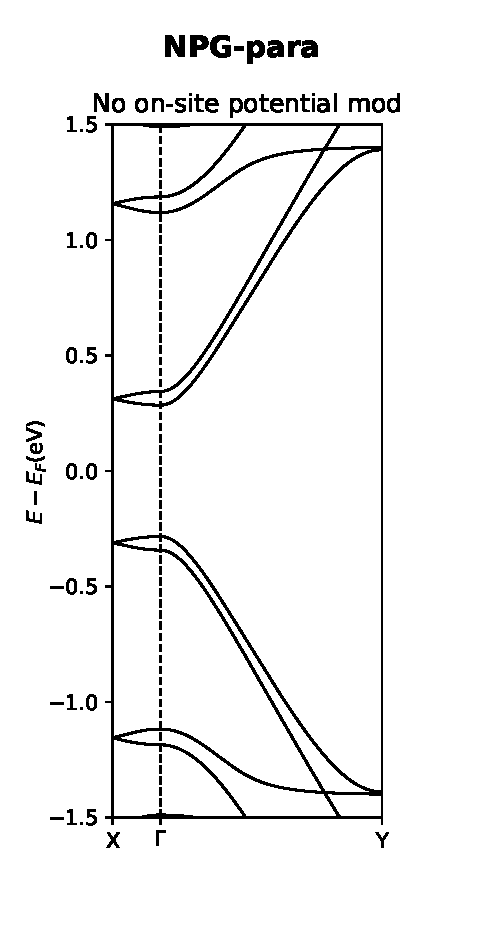
\includegraphics[width=\textwidth]{Figures/paraNPGBS.eps}
		\caption{Plot showing the band structure in the energy range \SI{-1.5}{\electronvolt} to \SI{1.5}{\electronvolt} for NPG with para bridges between symmetry points \(X\) and \(Y\) with respect to \(\Gamma\)}
		\label{parabs}
	\end{subfigure}
	~ %add desired spacing between images, e. g. ~, \quad, \qquad, \hfill etc.
	%(or a blank line to force the subfigure onto a new line)
	\begin{subfigure}[b]{0.3\textwidth}
		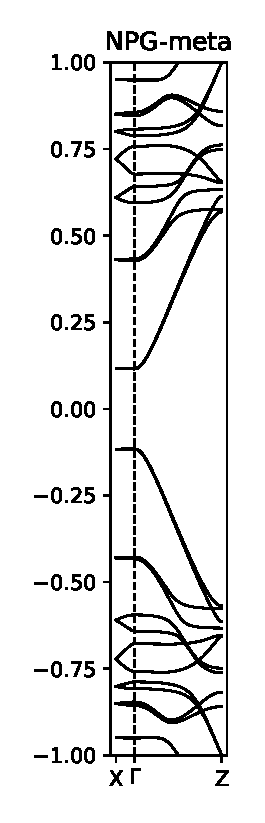
\includegraphics[width=\textwidth]{Figures/metaNPGBS.eps}
		\caption{Plot showing the band structure in the energy range \SI{-1.5}{\electronvolt} to \SI{1.5}{\electronvolt} for NPG with meta bridges between symmetry points \(X\) and \(Y\) with respect to \(\Gamma\)}
		\label{metabs}
	\end{subfigure}
	\caption{Figure showing para, meta and normal NPG band structures}\label{allbands}
\end{figure}
\im{Listings/Functions.py}{41}{47}
\vspace{-1\baselineskip}
\captionof{listing}{Function creating the hopping matrices between two sets of coordinates \label{hopfunc}}\vspace{\baselineskip}

\begin{figure}
	\centering
	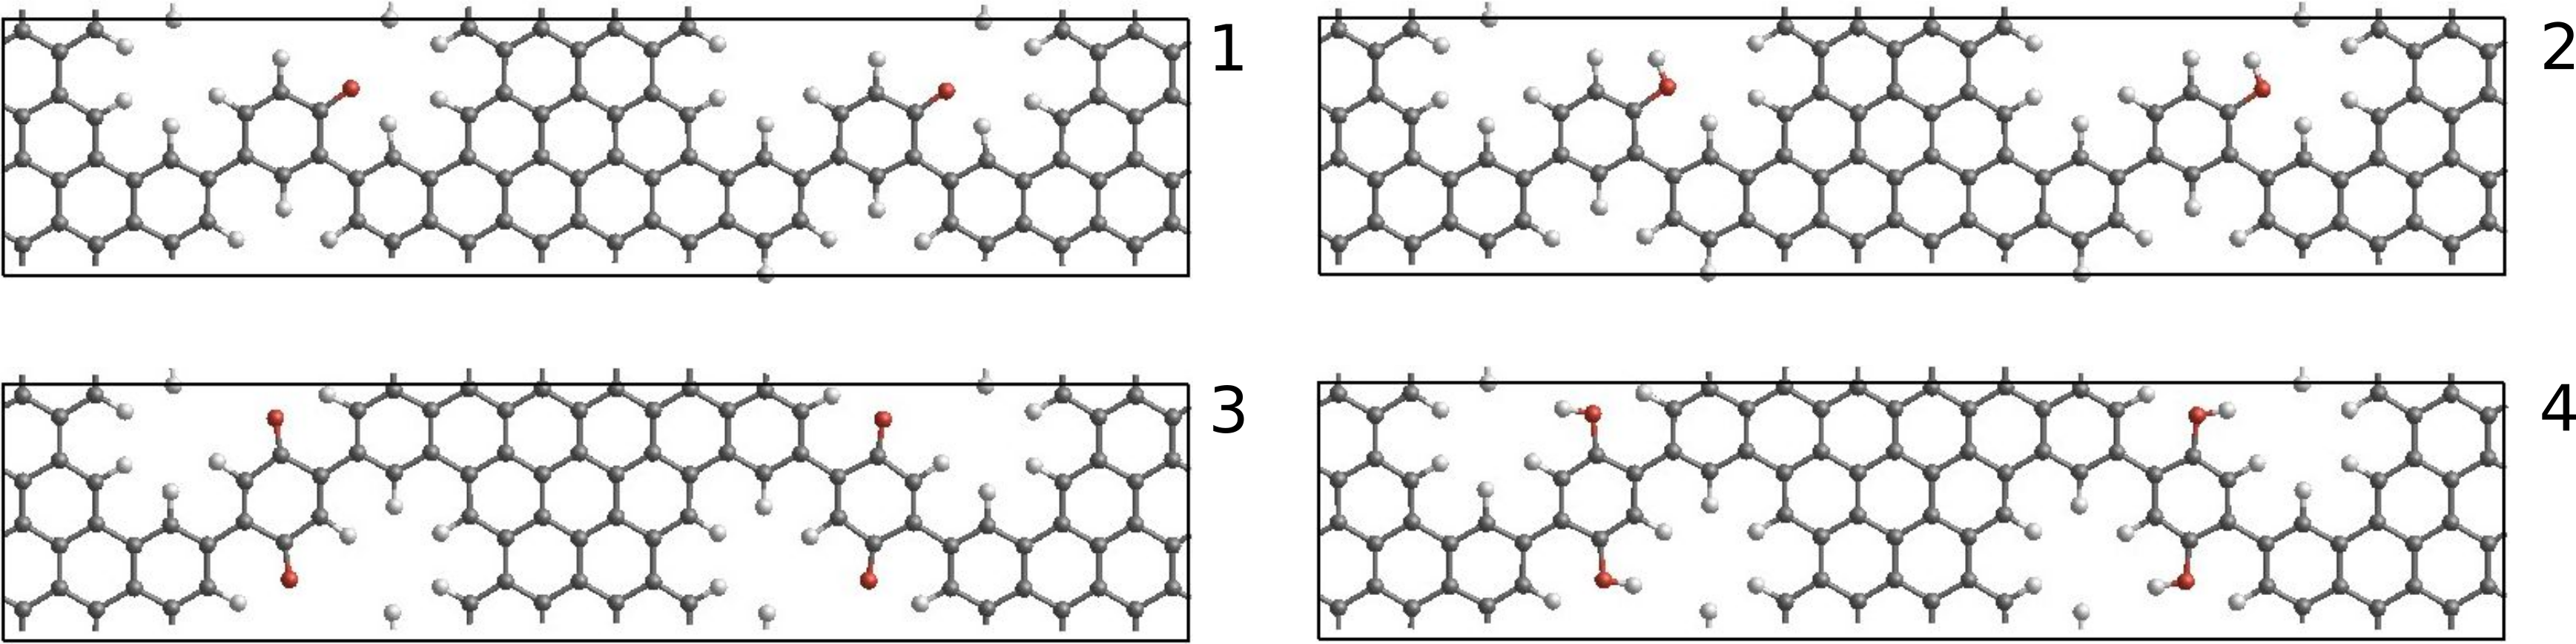
\includegraphics[width=\textwidth]{Figures/Structures.png}
	\caption{Figure showing all the structures stated in \cref{testtable}.}
	\label{Strucow}
\end{figure}

\im{Listings/Functions.py}{245}{252}
\vspace{-1\baselineskip}
\captionof{listing}{Code piece showing how the periodic Hamiltonian, shifted in the transverse direction i created using the given unit vector in the y direction.}{\label{periodichamilcode}}\vspace{\baselineskip}

\im{Listings/Functions.py}{234}{242}
\vspace{-1\baselineskip}
\captionof{listing}{Code piece showing how the transmission per energy point, using equation \cref{}.}{\label{transmissioncode}}\vspace{\baselineskip}

% \section{Project overview}
% A Gantt chart is provided on the next page. \textbf{Not Updated.}
% \newpage
% \begin{turnpage}
% \setcounter{myWeekNum}{6}
% \ganttset{%
% 	calendar week text={\myWeek{}}%
% }
% \begin{figure}\vspace{-10mm}
% \begin{ganttchart}[
% 		hgrid,
% 		vgrid={*{6}{draw=none}, dotted},
% 		x unit=.15cm,
% 		%	y unit title=.6cm,
% 		%	y unit chart=.6cm,
% 		inline,
% 		milestone inline label node/.append style={left=5mm},
% 		milestone/.append style={xscale=3},
% 		time slot format=isodate,
% 		time slot format/start date=2019-02-04
% 	]{2019-02-04}{2019-05-31}
% 	\gantttitlecalendar{year, month=shortname, week}\\
% 	\ganttgroup{Report writing}{2019-02-25}{2019-05-31}\\
% 	\ganttgroup[inline = false]{Course 33442}{2019-02-04}{2019-03-31}\\
% 	\ganttbar{Ch. 1 \& 2}{2019-02-04}{2019-02-17}\\
% 	\ganttlinkedbar[link bulge=2]{Ch. 3}{2019-02-18}{2019-02-24}\\
% 	\ganttlinkedbar[link bulge=2,bar inline label node/.style={right=15pt}]{Ch. 4 \& 5}{2019-02-25}{2019-03-03}\\
% 	\ganttgroup[inline = false]{Python code}{2019-03-04}{2019-03-31}\\
% 	\ganttbar{Py TB scripts}{2019-02-18}{2019-03-17}\\
% 	\ganttlinkedbar[link bulge=2, bar inline label node/.style={right=45pt}]{Small NPG systems simulations}{2019-03-10}{2019-03-31}\\
% 	\ganttmilestone{Proof of Concept with Python}{2019-03-31}\\
% 	\ganttgroup[inline = false]{Large scale TB}{2019-04-01}{2019-04-28}\\
% 	\ganttbar[bar inline label node/.style={left=10pt}]{SISL \& TBtrans tutorial}{2019-04-01}{2019-04-05}\\
% 	\ganttlinkedbar[link bulge=2, bar inline label node/.style={right=50pt}]{Setup NPG variations}{2019-04-06}{2019-04-28}\\
% 	\ganttgroup[inline = false]{Generate data}{2019-04-28}{2019-05-31}\\
% 	\ganttmilestone{Hand in report}{2019-05-31}
% \end{ganttchart}
% \end{figure}
% \end{turnpage}
% \clearpage
% \global\pdfpageattr\expandafter{\the\pdfpageattr/Rotate 90}

\end{document}
